\section{Exerciţii recapitulative}

\begin{enumerate}
\item
Fie limbajul: \textit{Toate succesiunile de caractere formate pe baza caracterelor a şi b care încep cu a, se termină cu b şi conţin subşirul abc}.
\begin{enumerate}
\item 
Construiţi o gramatică care să definească acest limbaj.	
\item 
Având în vedere ierarhia Chomsky, precizaţi cărora dintre tipuri corespunde gramatica definită şi explicaţi de ce.
\item 
Alegeţi o propoziţie care aparţine acestui limbaj şi o propoziţie care nu aparţine acestui limbaj. Scrieţi succesiunea de derivări directe care pot fi folosite pentru a genera propoziţiile pornind de la simbolul de start. Explicaţi.
\item 
Construiţi arborii de derivare (arborele ascendent şi arborele descendent) pentru propoziţia de la punctul 3. Explicaţi.
\end{enumerate}

\begin{itemize}
\item[a)]
$G = (V_{N}, \Sigma, S, P)$

$V_{N}= \{N, Y, B\}$

$\Sigma = \{$a, b, c$\} $ 

$S = N$

$P=\{$

$(1,2,3,4) \; N \rightarrow a Y B Y b | a B Y b | a Y B b | a B b$

$(5,6,7,8,9,10) \; Y \rightarrow a Y | b Y | c Y | a | b | c$

$(11) \; B \rightarrow abc $

$\}$

\item[b)] 
Gramatica este o gramatică de tipul al 2-lea (gramatică independentă de context), deoarece toate regulile de producţie din mulţimea $P$ a gramaticii, au forma $A \rightarrow \alpha$, unde $A \in V_N$, iar $\alpha \in V^*$.

\item[c)] 
\begin{itemize}
\item $aabaabcb \in L(G)$

Derivare stânga: $ N \Rightarrow^3  a Y B b \Rightarrow^5$ $a a Y B b$ $ \Rightarrow^6 $ $a a b Y B b$ $\Rightarrow^8$ $a a b a B b$ $\Rightarrow^{11} aabaabcb$ $\Leftrightarrow$ $aabaabcb$ $\in L(G)$

Derivare dreapta: $ N \Rightarrow^3 a Y B b$ $\Rightarrow^{11} a Y abc b$ $\Rightarrow^5 a a Y abc b$ $ \Rightarrow^6 a a b Y abc b$ $\Rightarrow^8 a a b a abc b$ $\Leftrightarrow a a b a abc b \in L(G)$

\item $ab \notin L(G)$

$N \Rightarrow^4 a B b \Leftrightarrow$ $ab$ $\notin L(G)$

Nu există nicio succesiune de derivări care să ducă la obţinerea propoziţiei $ab$.
\end{itemize}

\item[d)]
Arborele descendent este reprezentat în Figura \ref{probleme1ar1}. Arborele ascendent este reprezentat în Figura \ref{probleme1ar2}.

\begin{figure}[H]
\centering
\begin{tikzpicture}
\node {$N$}
child { node {$a$} }
child { node {$Y$} 
	child { node {$a$} }
    child { node {$Y$} 
		child { node {$b$} }    
		child { node {$Y$} 
			child { node {$a$} }		
		}
    }
}
child[missing] {}
child { node{$B$} 
	child { node {$a$} }
	child { node {$b$} }
	child { node {$c$} }
}
child { node{$b$} };
\end{tikzpicture}
\caption{Arborele sintactic descendent}
\label{probleme1ar1}
\end{figure}

\begin{figure}[H]
\centering
\begin{tikzpicture}[grow'=up]
\tikzset{frontier/.style={distance from root=150pt}}
\node {$N$}[grow'=up]
child { node {$a$} }
child { node {$Y$} 
	child { node {$a$} }
    child { node {$Y$} 
		child { node {$b$} }    
		child { node {$Y$} 
			child { node {$a$} }		
		}
    }
}
child[missing] {}
child { node{$B$} 
	child { node {$a$} }
	child { node {$b$} }
	child { node {$c$} }
}
child { node{$b$} };
\end{tikzpicture}
\caption{Arborele sintactic ascendent}
\label{probleme1ar2}
\end{figure}
\end{itemize}

\item
Fie limbajul: \textit{Toate succesiunile de caractere formate pe baza caracterelor a şi b care conţin subşirul ab sau subşirul ba}. Aceleaşi cerinţe ca şi la problema anterioară.

\begin{enumerate}
\item[a)]
$G = (V_{N}, \Sigma, S, P)$

$V_{N}= \{N, Y, Z\}$

$\Sigma = \{$a, b$\} $ 

$S = N$

$P=\{$

$(1,2,3) \; N \rightarrow a N | b N | Y$

$(4,5) \; Y \rightarrow ab Z | ba Z$

$(6,7,8,9) \; Z \rightarrow aZ | bZ | a | b$

$\}$

\item[b)]
Gramatica este o gramatică de tipul al 3-lea (gramatică regulată), deoarece toate regulile de producţie din mulţimea $P$ a gramaticii, au forma $A \rightarrow x B$ sau $A \rightarrow x$, unde $A,B \in V_N$, iar $x \in \Sigma^*$.

\item[c)]
\begin{itemize}
\item
$aabab \in L(G)$:

Derivare stanga:

$N \Rightarrow^1 a N \Rightarrow^1 a a N \Rightarrow^3 a a Y \Rightarrow^5 a a ba Z \Rightarrow^9 a a ba b$ $\Leftrightarrow aabab \in L(G)$

Derivare dreapta: Deoarece gramatica este o gramatică regulată, derivarea dreapta coincide cu derivarea stânga, adică au acelaşi număr de paşi (pentru a ajunge de la simbolul de start la propoziţie), iar formele propoziţionale intermediare sunt identice, pentru fiecare pas în parte.

$aaa$

Derivare stanga:

$N \Rightarrow a N \Rightarrow a a N \Rightarrow a a a N \Leftrightarrow aaa \notin L(G)$

Derivare dreapta: Aceeaşi observaţie ca şi mai sus.

\end{itemize}

\item[d)]
Pentru propoziţia $aabab$, arborele descendent este ilustrat in Figura \ref{}, iar arborele ascendent este ilustrat in Figura \ref{}.

\begin{figure}[H]
\begin{tikzpicture}
\node {S}
child {node {G} 
  child{node{G}
   child {node {L}
	child{node{B}  child{node{a}}}
	child{node{L} child{node{ab}}}}}
  child{node{L}  child{node{ab}}}};
\end{tikzpicture}
\caption{Arborele sintactic descendent}
\end{figure}

\begin{figure}[h!]
\begin{tikzpicture}[grow'=up]
\node {S}
child {node {G} 
  child{node{G}
   child {node {L}
	child{node{B}  child{node{a}}}
	child{node{L} child{node{ab}}}}}
  child{node{L}  child{node{ab}}}};
\end{tikzpicture}
\caption{Arborele sintactic ascendent}
\end{figure}

\end{enumerate}

\item
Fie limbajul: \textit{Toate succesiunile de caractere formate pe baza caracterelor u şi v care conţin subşirurile uu şi vv, în această ordine}. Aceleaşi cerinţe ca şi la problema anterioară.

\begin{enumerate}
\item[a)]
Gramatica generatoare pentru acest limbaj este:
\begin{itemize}
\item $\Sigma = \{ u,v\}$
\item S simbol de start
\item $P=\{ S\rightarrow CuuCvvC \newline 
C\rightarrow uL_{v}|vL_{v}|vL_{u}|\epsilon \newline
L_{v}\rightarrow v|vL_{u}|vL_{v}|\epsilon \newline
L_{u}\rightarrow u|uL_{v}|\epsilon \}$
\item $V_{N}=\{S, C, L_{u}, L_{v}\}$
\end{itemize}

\item[b)]
Avand in vedere ierarhia Chomsky putem spune ca gramatica este una de tip 2, gramatica independenta de context.Dupa cum spune definitia aceste gramatici sunt definite de niste reguli de productie ce au in stanga un neterminal iar in dreapta o serie de terminale si neterminale.

\item[c)]
\begin{itemize}
\item \textbf{uvvuvuuvuvv}\newline
\textbf{S} $\rightarrow$ CuuCvv\textbf{C} $\rightarrow$ CuuCvv\textbf{$\epsilon$} $\rightarrow$ Cuu\textbf{C}vv $\rightarrow$ Cuuv\textbf{$L_{u}$}vv $\rightarrow$ \textbf{C}uuvuvv $\rightarrow$ u\textbf{$L_{v}$}uuvuvv $\rightarrow$ uv\textbf{$L_{v}$}uuvuvv $\rightarrow$ uvv\textbf{$L_{u}$}uuvuvv $\rightarrow$ uvvu\textbf{$L_{v}$}uuvuvv $\rightarrow$ uvvuvuuvuvv \newline
Avand in vedere ca am obtinut secventa ceruta urmand regulile de productie aceasta apartine limbajului.
\item \textbf{uvuvvuuv}\newline
\textbf{S} \newline
Avand in vedere ca nu putem forma secventa ceruta urmand regulile de productie aceasta este respinsa de limbaj.
\end{itemize}
\item Reprezentarea derivarilor la stanga si la dreapta sub forma de arbore ascendent respectiv descendent este:

\begin{figure}[H]
\tikzstyle{level 1}=[level distance=1.5cm, sibling distance=5em]
\tikzstyle{level 2}=[level distance=1.5cm, sibling distance=1.5cm]
% definire stil pentru bag si end
\tikzstyle{bag} = [text width=2em, text centered]
\tikzstyle{end} = [circle, minimum width=1pt,fill, inner sep=0pt]
\begin{tikzpicture}[grow=up, sloped]
\node[bag] {S}
child {node[bag] {C}
	   child{node[bag] {$\epsilon$}}
      }
child {node[bag] {vv}}
child {node[bag] {C}
	   child{node[bag] {$L_{u}$}
	   		 child{node[bag] {u}}
	   		}
	   child{node[bag] {v}}
      }
child {node[bag] {uu}}
child {node[bag] {C}
       child {node[bag]{$L_{v}$}
       		  child{node[bag] {$L_{v}$}
       		  		child{node[bag] {$L_{u}$}
       		  			  child{node[bag] {$L_{v}$}
       		  			  		child{node[bag] {v}}
       		  			  	   }
       		  			  child{node[bag] {u}}
       		  			 }
       		  		child{node[bag] {v}}
       		  	   }
       		  child{node[bag] {v}}
             }
	   child {node[bag]{u}}
      };
\end{tikzpicture}
\caption{Arbore ascendent pentru derivare la stanga ex.1.4}
\end{figure}

Derivare la stanga inseamna ca mereu se schimba , conform unei reguli de productie, neterminalul cel mai din stanga.\newline
Derivare la dreapta inseamna ca mereu se schimba tot conform unei reguli de productie insa neterminalul aflat cel mai in dreapta.\newline
Arbore ascendent inseamna ca se pleaca de la secventa data si se fac operatiile inverse de la regulile de productie, nu urmam sensul sagetii ci facem invers. \newline
Arbore descendent inseamna ca se pleaca de la simbolul de start si se urmaresc regulile de productie urmand ca pe nodurile frunza,citite de la stanga la dreapta, sa se construiasca secventa ceruta.

\begin{figure}[H]
\tikzstyle{level 1}=[level distance=1.5cm, sibling distance=5em]
\tikzstyle{level 2}=[level distance=1.5cm, sibling distance=1.5cm]
% definire stil pentru bag si end
\tikzstyle{bag} = [text width=2em, text centered]
\tikzstyle{end} = [circle, minimum width=1pt,fill, inner sep=0pt]
\begin{tikzpicture}[grow=down, sloped]
\node[bag] {S}
child {node[bag] {C}
	   child {node[bag]{u}}
       child {node[bag]{$L_{v}$}
       		  child{node[bag] {v}}
       		  child{node[bag] {$L_{v}$}
       		  		child{node[bag] {v}}
       		  		child{node[bag] {$L_{u}$}
       		  			  child{node[bag] {u}}
       		  			  child{node[bag] {$L_{v}$}
       		  			  		child{node[bag] {v}}
       		  			  	   }
       		  			 }
       		  	   }
             }
      }
child {node[bag] {uu}}
child {node[bag] {C}
	   child{node[bag] {v}}
	   child{node[bag] {$L_{u}$}
	   		 child{node[bag] {u}}
	   		}
      }
child {node[bag] {vv}}
child {node[bag] {C}
	   child{node[bag] {$\epsilon$}}
      };
\end{tikzpicture}
\caption{Arbore descendent pentru derivare la dreapta ex.1.4}
\end{figure}
\end{enumerate}

\item
Fie limbajul: \textit{Toate succesiunile de caractere formate pe baza caracterelor u şi v care conţin unul sau mai multe \textbf{subşiruri} de tipul uuv.} Aceleaşi cerinţe ca şi la problema anterioară.

\begin{enumerate}
\item[a)]
Gramatica:
\begin{itemize}
\item
$\Sigma$ = \{u, v\};
\item
$V_{N}$ = \{S, G,Lc, C\};
\item
S $\rightarrow$ LcGLc | GLc | LcG | G;
\item
G $\rightarrow$ Guuv | uuv ;
\item
Lc $\rightarrow$ CLc | C;
\item
C $\rightarrow$ u|v;
\end{itemize}

\item[b)]
Gramatica definita este o gramatica de tipul 3 deoarece este o gramatica regulata in care se aplica succesiv derivari stanga sau dreapta.Si este o gramatica finita deoarece este o reprzentare finita.

\item[c)]
Următorul şir de derivări, care reprezintă generarea propoziţiei \textit{uuuuuvvvv}, este format din derivări stânga.

$S \Rightarrow LcGLc \Rightarrow CLcGLc \Rightarrow uLcGLc \Rightarrow uCLcGLc \Rightarrow uuLcGLc \Rightarrow uuCGLc  \Rightarrow uuuGLc \Rightarrow uuuuuvLc \Rightarrow uuuuuvCLc \Rightarrow uuuuuvvLc \Rightarrow uuuuuvvCLc \Rightarrow uuuuuvvvLc \Rightarrow uuuuuvvvC \Rightarrow uuuuuvvvv $

Următorul şir de derivări, care reprezintă generarea propoziţiei \textit{uvuuvuuvvu}, este format din derivări dreapta.

$S \Rightarrow LcGLc \Rightarrow LcGCLc \Rightarrow LcGCC \Rightarrow LcGuuvCC \Rightarrow CLcGuuvCC \Rightarrow CCGuuvCC \Rightarrow CCGuuvCu \Rightarrow CCGuuvvu \Rightarrow CCuuvuuvvu \Rightarrow Cvuuvuuvvu \Rightarrow uvuuvuuvvu  $

\item[d)]
\textbf{Arborele descendent} pentru derivare stanga$\rightarrow$pornim de la nodul de start si obtinem propozitia.

\begin{figure}[H]
\begin{tikzpicture}
\centering
\node {S} [sibling distance=3.5cm ]
    child { node {Lc} [sibling distance=3cm ]
	child{node {C}
		child{node{uuv}}}
          child{node{Lc}[sibling distance=2cm]
		child{node{C}
			child{node{u}}}
		child{node{Lc}
			child{node{C}
				child{node{u}}}}}}
    child{node{G}
	child{node{uuv}}}
    child{node{Lc}[sibling distance=3cm]
	child{node{C}
		child{node{v}}}
	child{node{Lc}[sibling distance=2cm]
		child{node{C}
			child{node{v}}}
		child{node{Lc}
			child{node{C}
				child{node{v}}}}}}
;
\end{tikzpicture}
\end{figure}

\textbf{Arborele ascendent} pentru derivare dreapta$\rightarrow$pornim de la frunze si obtinem nodul de start.\\\\

\begin{figure}[H]
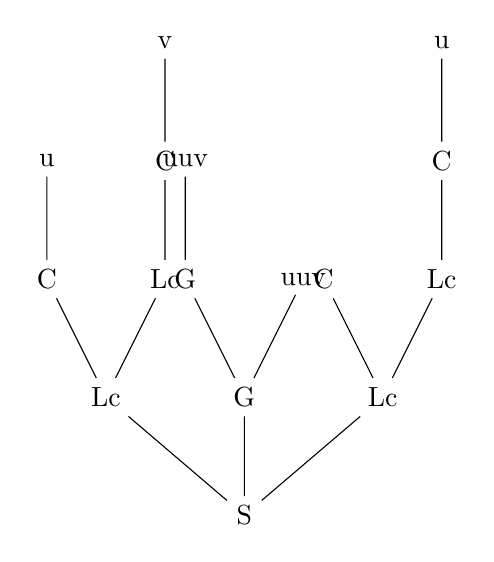
\begin{tikzpicture}
\node {S}[grow=up][sibling distance=3.5cm ]
child {node {Lc}[sibling distance=2cm]
	child{node{Lc}
		child{node{C}
			child{node{u}}}}
	child{node{C}} }
child{node{G}[sibling distance=2cm]
	child{node{uuv}}
	child{node{G}
		child{node{uuv}}}}
child{node{Lc}[sibling distance=2cm]
	child{node{Lc}
		child{node{C}
			child{node{v}}}}
	child{node{C}
		child{node{u}}}}
;
\end{tikzpicture}
\end{figure}

\end{enumerate}

\item
Fie limbajul: \textit{Toate succesiunile de caractere formate pe baza caracterelor 0 şi 1 care încep  cu cel puţin un 1 după care urmează doi de 0 şi apoi o succesiune oarecare de 0 şi 1.} Aceleaşi cerinţe ca şi la problema anterioară.

\begin{enumerate}
\item[a)]
Alfabetul limbajului (multimea terminalelor):  
$\Sigma = \{$0, 1$\}$ \\
Multimea neterminalelor:  
$V_N = \{N, L_A, L_B, A, B, Z\}$ \\
Simbolul de start: 
$S = N$ \\
Multimea regulilor de producie:

\begin{enumerate}
\item $N \rightarrow AL_AZL_B$
\item $L_A \rightarrow  AL_A \; | \; \epsilon$
\item $A \rightarrow 1$
\item $L_B \rightarrow BL_B \; | \;  \epsilon$
\item $B \rightarrow 0 \;|\; 1$
\item $Z \rightarrow 00$
\end{enumerate}

Verificare: subpunctul 3

\item[b)]
Gramatica este de tipul 2, deoarece regulile sale sunt de tipul $x \rightarrow r$ cu $x$ neterminal si $r$ un sir de terminali si neterminali ($x \in V_{N}, r \in V^{\ast}$). Aceasta este o gramatica libera, o gramatica independenta de context.

\item[c)]
\begin{itemize}
\item 11100010 $\in$ limbajului \\ \\
$ N \xRightarrow{(a)} AL_AZL_B \xRightarrow[(f),(d.1)]{(c),(b.1)} 1AL_A00BL_B \xRightarrow[(c)]{(e)} 11L_A000L_B \xRightarrow[(d.1)]{(b.1)} 11AL_A000BL_B \xRightarrow[(e),(d.1)]{(c)} 111L_A0001BL_B \xRightarrow[(e)]{(b.2)} 11100010L_B \xRightarrow{(d.2)} 11100010$     \;\; \checkmark \\
\item 100 $\in$ limbajului\\ \\
$N \xRightarrow{(a)} AL_AZL_B \xRightarrow[(c)]{(f)}1L_A00L_B \xRightarrow[(d.2)]{(b.2)} 100$  \;\; \checkmark
\item 001 \\ \\
$N \xRightarrow{(a)} AL_AZL_B \xRightarrow[(f)]{(c)} 1L_A00L_B$\;\; \checkmark \; nu se poate genera 001 $\notin$ limbajului
\end{itemize}

\item[d)]
Arborele ascendent pentru derivarea stânga (11100010)

\begin{figure}[H]
\centering
\begin{tikzpicture}
\node {N}[grow=up]
child {node {$L_B$}
	child {node {$L_B$}
		child {node {$L_B$}
			child {node {$L_B$}
				child {node {$\epsilon$}}}
			child {node{$B$}
				child {node {$0$}}}}
		child {node{$B$}
			child {node {$1$}}}}
	child {node {$B$}
		child {node {$0$}}}
}
child {node {$Z$}
   child {node {$00$}}
}
child {node {$L_A$}
	child {node {$L_A$}
		child {node {$L_A$}
			child {node {$\epsilon$}}}
		child {node{$A$}
			child {node {$1$}}}}
	child {node {$A$}
		child {node {$1$}}}
}
child {node {$A$} 
   child {node {$1$}}
};
\end{tikzpicture}
\end{figure}

Arborele ascendent se formeaza pornind de la frunze(propozitie) catre radacina şi identificând regulile de productie aplicate. Astfel se ajunge la simbolul de start. 

Arborele descendent pentru derivarea dreapta 11100010:\\ \\
$ N \xRightarrow{(a)} AL_AZL_B \xRightarrow[(d.1)]{(b.1)} AAL_AZBL_B \xRightarrow[(d.1)]{(b.1)} AAAL_AZBBL_B \xRightarrow[(d.1)]{(b)} AAAZBBBL_B \xRightarrow{(d.2)} AAAZBBB \xRightarrow[(e)]{(c),(f)} 11100010$\\

Arborele descendent se formeaza pornind de la radacina şi aplicand succesiv regulile de productie, frunze continand fiecare un element al limbajului. Astfel, putem citi de la stanga la dreapta 
frunzele arborelui pentru a reface propozitia de la care am plecat.

\begin{figure}[H]
\centering
\begin{tikzpicture}
\node {$N$}
[sibling distance=2cm]
child {node {$A$} 
   child {node {$1$}}
}
child {node {$L_A$}
	[sibling distance=1.3cm]
	child {node {$A$}
	   child {node {$1$}}}
	child {node {$L_A$}
		child {node {$A$}
		   child {node {$1$}}}
		child {node {$L_A$}
			child {node {$\epsilon$}}
		}
	}	
}
child {node {$Z$}
   child {node {$00$}}
}
child {node {$L_B$}
	[sibling distance=1.3cm]
	child {node {$B$}
	   child {node {$0$}}}
	child {node {$L_B$}
		child {node {$B$}
		   child {node {$1$}}}
		child {node {$L_B$}
			child {node {$B$}
		  		 child {node {$1$}}}
			child {node {$L_B$}
				child {node {$\epsilon$}}}	
		}
	}	
};
\end{tikzpicture}
\end{figure}

\end{enumerate}

\item
Fie limbajul: \textit{Toate succesiunile de caractere formate pe baza caracterelor a şi b care se termină cu a urmat de oricâţi de b şi apoi de un a.} Aceleaşi cerinţe ca şi la problema anterioară.

\begin{enumerate}
\item[a)]
$\Sigma=\{a,b\}$\\
N $\rightarrow$ AaBa\\
A $\rightarrow$ aA | bA | a | b \\
B$\rightarrow$ bB | b\\

\item[b)]
Gramatica definita este independenta de context deoarece este reprezentata ca reguli de forma A $\rightarrow$ $\gamma$ cu A neterminal si $\gamma$ un sir de terminali si neterminali. Aceste limbaje sunt exact toate limbajele care poti fi recunoscute de un automat cu stiva nedeterminist. Limbajele independente de context constituie baza teoretica a majoritatii limbajelor de programare.

\item[c)]
Apartine :  ababa
N $\rightarrow$ AaBa $\rightarrow$ aAaBa $\rightarrow$aAaBa $\rightarrow$ abaBa $\rightarrow$ ababa\\

Nu apartine : ababaa

N $\rightarrow$ AaBa $\rightarrow$ aAaBa $\rightarrow$aAaBa $\rightarrow$ abaBa $\rightarrow$ ababa $\Rightarrow$  ababaa nu apartine acestui limbaj

\item[d)]
Construiţi arborii de derivare (arborele ascendent pentru derivarea stânga şi arborele descendent pentru derivarea dreapta) pentru propoziţiile de la punctul 3. Explicaţi.

\begin{figure}
\centering
\begin{tikzpicture}
\node {N}[grow=up]
child {node {A}
    child {node {a}}
    child {node {b}}
    }
 child {node {a}}
child {node {B} 
   child {node {b}}
    }
 child {node {a}}
;
\end{tikzpicture}
\caption{Arborele sintactic ascendent pentru propoziţia \textit{ababa}}

\centering
\begin{tikzpicture}
\node {N}
child {node {A} 
  child {node {a}}
  child {node {b}}
}
child {node {a}}
child {node {B}
     child {node {b}}}
child {node {a}};
\end{tikzpicture}
\caption{Arborele sintactic descendent pentru propoziţia \textit{ababa}}
\end{figure}
\end{enumerate}

\item
Fie limbajul: \textit{Toate succesiunile de simboluri formate pe baza simbolurilor a, b şi c care începe cu cel puţin un grup bc, conţine maxim un grup cba şi se încheie cu cel puţin doi de a.} Aceleaşi cerinţe ca şi la problema anterioară.

\begin{itemize}
\item[a)]
$G = (V_{N}, \Sigma, S, P)$

$\Sigma = \{$a, b, c$\} $ 

$V_{N}= \{A, B, C, X\}$

$N \rightarrow AXBXC$

$A \rightarrow bc|bcA $

$B \rightarrow bca|\epsilon $

$C \rightarrow aaC|aa $

$X \rightarrow aX|bX|CY$

$Y \rightarrow aY|bM|cY|\epsilon$

$M \rightarrow aL|bM|cM|\epsilon$

$L \rightarrow bL|cL|\epsilon$
 
\item[b)]
Gramatica este de tip 2, deoarece este independenta de context si poate fi recunoscuta de un automat cu stiva.

\item[c)]
\begin{itemize}
\item $bcaa$
\\$N \Rightarrow AXBXC \Rightarrow bcXBXC \Rightarrow bc\epsilon BXC \Rightarrow bcBXC \Rightarrow bc \epsilon XC \Rightarrow bcXC \Rightarrow bc\epsilon C \Rightarrow bcC \Rightarrow bcaa  \Rightarrow$ propozitia $\in$ limbajului
\item $bcca$
\\$N \Rightarrow AXBXC \Rightarrow bcXBXC \Rightarrow bccBXC \Rightarrow bcc \epsilon XC \Rightarrow bccaC \Rightarrow $ nu se pot face derivari pentru C astfel incat sa se potriveasca $\Rightarrow$  propozotia $\notin$ limbajului.
\end{itemize}

\item[d)]
Vom deriva pentru propozitia $bc$ $cba$ $aa$
\\Derivare stanga:
\\$N \Rightarrow AXBXC \Rightarrow bcXBXC \Rightarrow bc \epsilon BXC bc BXC \Rightarrow bc cba XC \Rightarrow bc cba \epsilon C \Rightarrow bc cba C \Rightarrow bccbaC \Rightarrow bc$ $cba$ $aa$
\begin{figure}[h]
\centering
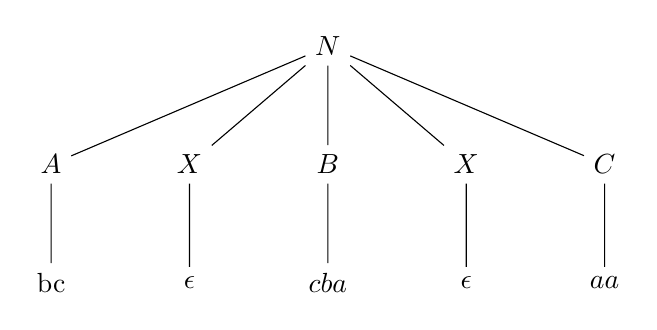
\begin{tikzpicture}
\node {$N$}
child { node {$A$}
		child {node{bc}} 
	  }	
child {node{$X $}
		child {node{$\epsilon$}}
		}
child { node{$B$}
		child { node {$cba$}}
	  }
child {node{$X$}
		child {node{$\epsilon$}}
	  }
child { node{$C$}
		child {node{$aa$}} };
\end{tikzpicture}
\caption{Arbore sintactic descendent derivare stanga}
\end{figure}

Derivare dreapta:
\\$N \Rightarrow ABC \Rightarrow ABaa \Rightarrow A cba aa \Rightarrow bccbaC \Rightarrow bc$ $cba$ $a$

\begin{figure}[h]
\centering
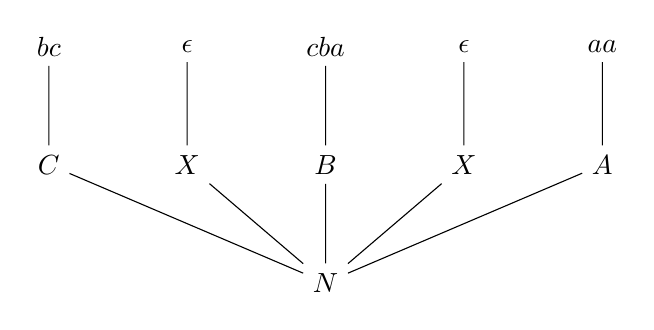
\begin{tikzpicture}
\node {$N$}[grow=up]
child { node {$A$}
		child {node{$aa$}} 
	  }	
child {node{$X $}
		child {node{$\epsilon$}}
		}	
child { node{$B$}
		child { node {$cba$}}
	  }
child {node{$X $}
		child {node{$\epsilon$}}
		}
child { node{$C$}
		child {node{$bc$}} };
\end{tikzpicture}
\caption{Arbore sintactic descendent derivare stanga}
\end{figure}
\end{itemize}

\item
Aceleaşi cerinţe ca şi problema anterioară, pentru limbajul: \textit{Toate succesiunile de simboluri formate pe baza simbolurilor a, b şi c care conţin cel puţin doi de b şi cel mult un c.}

\begin{enumerate}
\item[a)]
Gramatica:

$\sum=\{a,b,c\}$

Simbol de start:$S$

Multimea de neterminale: $V_N=\{G,L,A,B,C,D\}$

Reguli de productie:

$S \Rightarrow G$

$G \Rightarrow LBCL|LCBL|CLBL$

$L \Rightarrow A|B|D|L|\epsilon$

$B \Rightarrow Dbb|bbD$

$D \Rightarrow bD|\epsilon$

$A \Rightarrow aA|a$

$C \Rightarrow c|\epsilon$

\item[b)]
Conform ierarhiei Chomsky, gramatica definita la punctul 1 este independenta de context, fiind o gramatica formala sau generativa care descrie structural un limbaj peste $\sum$, iar fiecare regula de productie $\alpha \longrightarrow \beta$
 verifica $ \alpha \in V- \sum$, pentru $\beta \in V^\star$. Altfel spus, este de forma $A \longrightarrow u, A \in V_N$.

\item[c)]
Se considera exemplele:

$caabbbaa$

Prin derivare la stanga:

$S \longrightarrow G \longrightarrow CLBL \longrightarrow cLBL \longrightarrow cABL \longrightarrow caABL \longrightarrow caaBL \longrightarrow caaDbbL \longrightarrow caabDbbL \longrightarrow caab \epsilon bbL \longrightarrow caabbbL \longrightarrow caabbbA \longrightarrow caabbbaA \longrightarrow caabbbaa$

Prin derivare la dreapta:

$S  \longrightarrow G \longrightarrow CLBL \longrightarrow CLBA \longrightarrow CLBaA \longrightarrow CLBaa \longrightarrow CLbbDaa \longrightarrow CLbbbDaa \longrightarrow CLbbb \epsilon aa \longrightarrow CLbbbaa \longrightarrow CAbbbaa \longrightarrow CaAbbbaa \longrightarrow Caabbbaa \longrightarrow caabbbaa$

$aabcc$

Derivare la stanga:

$S  \longrightarrow G \longrightarrow LBCL \longrightarrow ABCL \longrightarrow aABCL \longrightarrow aaBCL \longrightarrow aaDbbCL$ ?? Propozitia nu apartine limbajului!

Derivare la dreapta:

$S \longrightarrow G \longrightarrow LBCL \longrightarrow LBC \epsilon \longrightarrow LBC \longrightarrow LBc \longrightarrow LDbbc$ ?? Propozitia nu apartine limbajului!

\item[d)]
Pentru exemplul "$caabbbaa$" arborele descendent este ilustrat in Figura 1.3, iar cel ascendent in Figura 1.4

\begin{figure}[H]
\begin{tikzpicture}[level 2/.style={sibling distance=5.7em},level 3/.style={sibling distance=1.8em},level 4/.style={sibling distance=2.3em}]
\node {S}
child {node {G} 
   child {node{C} child{node{c}}}
   child{node{L} 
	child{node{A} child{node{a}} child{node{A} child{node{a}}}}}
   child{node{B} 
	child{node{b}}
	child{node{b}}
	child{node{D}
		child{node{b}}
		child{node{D} child{node{$\epsilon$}}}}}
 child{node{L}
    	child{node{A}
		child{node{a}}
		child{node{A}  child{node{a}}}}}};
\end{tikzpicture}
\caption{Arborele descendent}
\end{figure}

\begin{figure}[H]
\begin{tikzpicture}[grow'=up,level 2/.style={sibling distance=5.7em},level 3/.style={sibling distance=1.8em},level 4/.style={sibling distance=2.3em}]
\node {S}
child {node {G} 
   child {node{C} child{node{c}}}
   child{node{L} 
	child{node{A} child{node{a}} child{node{A} child{node{a}}}}}
   child{node{B} 
	child{node{b}}
	child{node{b}}
	child{node{D}
		child{node{b}}
		child{node{D} child{node{$\epsilon$}}}}}
 child{node{L}
    	child{node{A}
		child{node{a}}
		child{node{A}  child{node{a}}}}}};
\end{tikzpicture}
\caption{Arborele ascendent}
\end{figure}

\end{enumerate}

\item
Aceleaşi cerinţe ca şi la problema anterioară, pentru limbajul: \textit{Toate succesiunile de simboluri formate pe baza simbolurilor a, b şi c care încep cu abc, conţin cel puţin un grup bb şi se termină cu a sau cu c.}

\begin{enumerate}
\item[a)]
\begin{itemize}
\item
$\Sigma$ = \{a,b,c\};
\item
$V_{N}$ = \{S, M,N,B,F,Lc\};
\item
S $\rightarrow$ MNF;
\item
N $\rightarrow$ LcBLc |  LcB | BLc | B ;
\item
Lc $\rightarrow$ FLc | F;
\item
M $\rightarrow$ abc;
\item
B $\rightarrow$ bb;
\item
F $\rightarrow$ a | c;
\end{itemize}

\item[b)]
Gramatica definita este o gramatica de tipul 3 deoarece este o gramatica regulata in care se aplica succesiv derivari stanga sau dreapta.Si este o gramatica finita deoarece este o reprzentare finita.

\item[c)]
abcbbc
Derivare stanga:
S$\rightarrow  MNF  \rightarrow abcNF  \rightarrow abcBF \rightarrow abcbbF  \rightarrow abcbbc$ (am consumat toate simbolurile => propozitia apartine limbajului)\\\\
Exemplul12: (abccbbca)\\\\
Derivare dreapta:
S$\rightarrow  MNF  \rightarrow MLcBLcF  \rightarrow M \rightarrow MLcBFF  \rightarrow MFBFF  \rightarrow abccbbca$ (am consumat toate simbolurile => propozitia apartine limbajului)\\\\\\

\item[d)]
\textbf{Arborele descendent} pentru derivare stanga$\rightarrow$pornim de la nodul de start si obtinem propozitia.\\\\

\begin{figure}[H]
\begin{tikzpicture}
  \node {S} [sibling distance=4cm ]
 child { node {M} [sibling distance=2cm ]
	child{node {abc}}}
 child {node{N}
	child{node {B} 
		child{node{bb} }}}
child {node{F}
	child {node{c}}};
\end{tikzpicture}
\end{figure}

Arborele ascendent pentru derivare dreapta$\rightarrow$pornim de la frunze si obtinem nodul de start.

\begin{figure}[H]
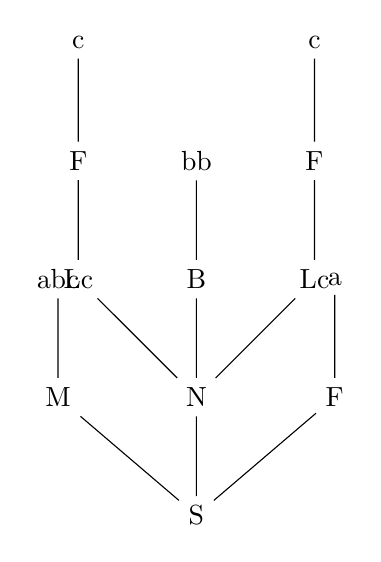
\begin{tikzpicture}
\node {S}[grow=up][sibling distance=5cm ]
child {node {F}
	child{node{a}}}
child{node{N}[sibling distance=2cm]
	child{node{Lc}
		child{node{F}
			child{node{c}}}}
	child{node{B}
		child{node{bb}}}
	child{node{Lc}
		child{node{F}
			child{node{c}}}}}
child{node{M}
	child{node{abc}}};
\end{tikzpicture}
\end{figure}

\end{enumerate}

\item
Aceleaşi cerinţe ca şi la problema anterioară, pentru limbajul: \textit{Toate succesiunile de simboluri formate pe baza simbolurilor a, b şi c care au lungimea cel puţin egală cu 3, iar al treilea simbol este a.}

\begin{enumerate}
\item[a)]
Gramatica generatoare pentru acest limbaj este:
\begin{itemize}
\item $\Sigma = \{ a,b,c\}$
\item S simbol de start
\item $P=\{ S \rightarrow C_{o}C_{o}aL \newline 
C_{o} \rightarrow a|b|c \newline
L \rightarrow CL|C \newline
C \rightarrow a|b|c|\epsilon  \}$
\item $V_{N}=\{S, C_{o}, L, C\}$
\end{itemize}

\item[b)]
Avand in vedere ierarhia Chomsky putem spune ca gramatica este una de tip 2, gramatica independenta de context.Dupa cum spune definitia aceste gramatici sunt definite de niste reguli de productie ce au in stanga un neterminal iar in dreapta o serie de terminale si neterminale.

\item[c)]
\begin{itemize}
\item \textbf{abaabc}\newline
\textbf{S} $\rightarrow$ \textbf{$C_{o}$}$C_{o}$aL $\rightarrow$ a\textbf{$C_{o}$}aL $\rightarrow$ aba\textbf{L} $\rightarrow$ aba\textbf{C}L $\rightarrow$ abaa\textbf{L} $\rightarrow$ abaa\textbf{C}L $\rightarrow$ abaab\textbf{L} $\rightarrow$ abaab\textbf{C} $\rightarrow$ abaabc \newline
Avand in vedere ca am obtinut secventa ceruta urmand regulile de productie aceasta apartine limbajului.
\item \textbf{ba}\newline
\textbf{S} $\rightarrow$ $C_{o}C){o}aL$ \newline
Avand in vedere ca nu putem trece din $C_{o}$ in $\epsilon$ secventa nu poate fi creata, cu alte cuvinte nu este acceptata de limbaj.
\end{itemize}

\item[d)]
Reprezentarea derivarilor la stanga si la dreapta sub forma de arbore ascendent respectiv descendent este:\newline
Explicatiile de la exercitiul anterior sunt valabile si pentru acesta.

\begin{figure}[H]
\tikzstyle{level 1}=[level distance=1cm, sibling distance=5em]
\tikzstyle{level 2}=[level distance=1cm, sibling distance=1.5cm]
% definire stil pentru bag si end
\tikzstyle{bag} = [text width=2em, text centered]
\tikzstyle{end} = [circle, minimum width=1pt,fill, inner sep=0pt]
\begin{tikzpicture}[grow=up, sloped]
\node[bag] {S}
child {node[bag] {L}
	   child{node[bag] {L}
	   		 child{node[bag] {L}
	   		 	   child{node[bag] {C}
	   		 	   		 child{node[bag] {c}}
	   		 	   		}
	   		 	  }
	   		 child{node[bag] {C}
	   		 	   child{node[bag] {b}}
	   		 	  }
	   		}
	   child{node[bag] {C}
	   		 child{node[bag] {a}}
	   		}
      }
child {node[bag] {a}}
child {node[bag] {$C_{o}$}
	   child{node[bag] {b}}
	   }
child {node[bag] {$C_{o}$}
       child {node[bag]{a}}
      };
\end{tikzpicture}
\caption{Arbore ascendent pentru derivare la stanga ex.2.4}
\end{figure}

\begin{figure}[H]
\tikzstyle{level 1}=[level distance=1.5cm, sibling distance=5em]
\tikzstyle{level 2}=[level distance=1.5cm, sibling distance=1.5cm]
% definire stil pentru bag si end
\tikzstyle{bag} = [text width=2em, text centered]
\tikzstyle{end} = [circle, minimum width=1pt,fill, inner sep=0pt]
\begin{tikzpicture}[grow=down, sloped]
\node[bag] {S}
child {node[bag] {$C_{o}$}
	   child{node[bag] {a}}
	   }
child {node[bag] {$C_{o}$}
       child {node[bag]{b}}
      }
child {node[bag] {a}}
child {node[bag] {L}
	   child{node[bag] {C}
	   		 child{node[bag] {a}}
	   		}
	   child{node[bag] {L}
	   		 child{node[bag] {C}
	   		 	   child{node[bag] {b}}
	   		 	  }
	   		 child{node[bag] {L}
	   		 	   child{node[bag] {C}
	   		 	   		 child{node[bag] {c}}
	   		 	   		}
	   		 	  }
	   		}
      }
;
\end{tikzpicture}
\caption{Arbore descendent pentru derivare la dreapta ex.2.4}
\end{figure}
\end{enumerate}

\item
Aceleaşi cerinţe ca şi la problema anterioară, pentru limbajul: \textit{Toate succesiunile de simboluri formate pe baza simbolurilor a, b şi c care încep cu a sau cu b, conţin subşirurile ac şi bc şi se termină cu un c sau cu doi de c.}

\begin{enumerate}
\item[a)]
$\Sigma=\{a,b,c\}$\\
N $\rightarrow$ ABC\\
A $\rightarrow$ a | b \\
B$\rightarrow$ D E D F D B | D E D F D | D F D E D B | D F D E D \\
C$\rightarrow$ c | cc\\
D$\rightarrow$ aD | bD | cD | a | b | c | $\epsilon$\\
E$\rightarrow$ acE | ac\\
F$\rightarrow$ bcF | bc\\

\item[b)]
Gramatica definita este independenta de context deoarece este reprezentata ca reguli de forma A $\rightarrow$ $\gamma$ cu A neterminal si $\gamma$ un sir de terminali si neterminali. Aceste limbaje sunt exact toate limbajele care poti fi recunoscute de un automat cu stiva nedeterminist. Limbajele independente de context constituie baza teoretica a majoritatii limbajelor de programare. \\

\item[c)]
Apartine :  abcacc\\
N $\rightarrow$ ABC $\rightarrow$ aBC $\rightarrow$aDFDEDC $\rightarrow$ aFDEDC $\rightarrow$ abcDEDC $\rightarrow$ abcEDC $\rightarrow$ abcacDC $\rightarrow$ abcacC $\rightarrow$  abcacc $\Rightarrow$ apartine acestui limbaj \\
\\
Nu apartine : abcac\\

N $\rightarrow$ ABC $\rightarrow$ aBC $\rightarrow$aDFDEDC $\rightarrow$ aFDEDC $\rightarrow$ abcDEDC $\rightarrow$ abcEDC $\rightarrow$ abcacDC $\rightarrow$ abcacC  $\Rightarrow$ nu apartine acestui limbaj

\item[d)]

\begin{figure}[H]
\centering
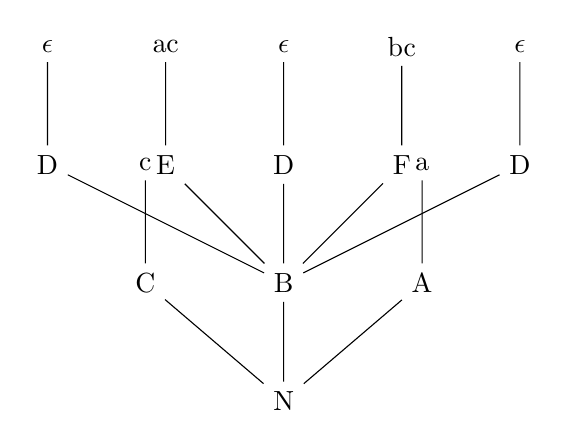
\begin{tikzpicture}
\node {N}[grow=up][sibling distance=9em] 
 child {node {A} 
child {node {a}}
}
    child {node {B} [sibling distance=3.8em]  
        child {node {D}
	child {node {$\epsilon$}}}
	child {node {F}
	child {node {bc}}}
	child {node {D}
	child {node {$\epsilon$}}}
	child {node {E}
	child {node {ac}}}
	child {node {D}
	child {node {$\epsilon$}}}
}  
	child {node {C}   
	child {node {c}}};
\end{tikzpicture}
\caption{Arborele sintactic ascendent pentru propoziţia \textit{abcacc}}
\centering
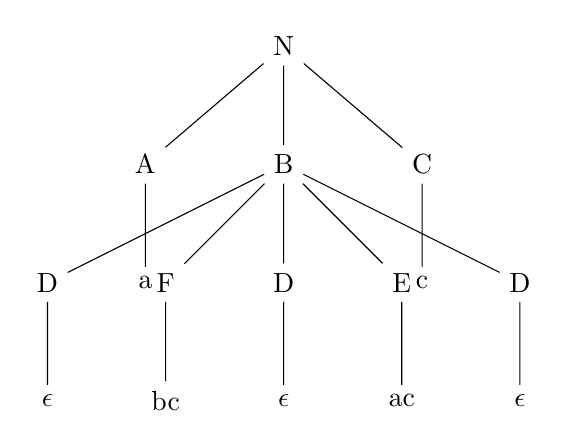
\begin{tikzpicture}
\node {N} [sibling distance=9em] 
child {node {A} 
  child {node {a}}}
  child {node {B}  [sibling distance=3.8em]  
        child {node {D}
	child {node {$\epsilon$}}}
	child {node {F}
	child {node {bc}}}
	child {node {D}
	child {node {$\epsilon$}}}
	child {node {E}
	child {node {ac}}}
	child {node {D}
	child {node {$\epsilon$}}}}
child {node {C}   
     child {node {c}}};
\end{tikzpicture}
\caption{Arborele sintactic descendent pentru propoziţia \textit{abcacc}}
\end{figure}

\end{enumerate}

\item
Aceleaşi cerinţe ca şi la problema anterioară, pentru limbajul: \textit{Toate succesiunile de simboluri formate pe baza simbolurilor a, b şi c care încep cu bc, conţin subşirul ac sau subşirul bc şi se termină cu cel puţin un grup aa.}

\begin{enumerate}
\item[a)]
Alfabetul limbajului (multimea terminalelor):  
$\Sigma = \{a, b, c\}$ \\
Multimea neterminalelor:  
$V_N = \{N, M, P, Q, R, S\}$ \\
Simbolul de start: 
$S = N$ \\
Multimea regulilor de producie:

\begin{enumerate}
\item $N \rightarrow MPQR$
\item $M \rightarrow  bc$
%\item $S \rightarrow LPL$
\item $P \rightarrow ac \;|\; bc$
%\item $L \rightarrow AL \;|\; \epsilon$
%\item $A \rightarrow a\;|\;b\;|\;c$
\item $R \rightarrow QR \; | \;  \epsilon$
\item $Q \rightarrow aa$
\end{enumerate}

Verificare: subpunctul 3

\item[b)]
Gramatica este de tipul 2, deoarece regulile sale sunt de tipul $x \rightarrow r$ cu $x$ neterminal si $r$ un sir de terminali si neterminali ($x \in V_{N}, r \in V^{\ast}$). Aceasta este o gramatica libera, o gramatica independenta de context.

\item[c)]
\begin{itemize}
\item bcbcaaaa $\in$ limbajului \\ 
$ N \xRightarrow{(a)} MPQR \xRightarrow[(e),(d)]{(c),(b)} bcbcaaQR \xRightarrow[(d.2)]{(h)} bcbcaaaa$     \;\; \checkmark \\
\item bcacaa $\in$ limbajului\\ 
$N \xRightarrow{(a)}MPQR \xRightarrow[(e),(d.2)]{(b),(c)} bcacaa$  \;\; \checkmark
\item bcaaaabc $\notin$ limbajului\\ 
$N \xRightarrow{(a)}MPQR \xRightarrow[(e)]{(b} bcPaa$  \;\; \checkmark  \; nu se poate genera 001 $\notin$ limbajului

\end{itemize}

\item[d)]
Arborele ascendent pentru derivarea stânga (11100010)

\begin{figure}
\centering
\begin{tikzpicture}
\node {N}[grow=up]
child {node {$R$}
	child {node {$R$}
		child {node {$\epsilon$}}}
	child {node {$Q$}
		child {node {$aa$}}}
}
child {node {$Q$}
   child {node {$aa$}}
}
child {node {$P$}
	child {node {$bc$}}
}
child {node {$M$} 
   child {node {$bc$}}
};
\end{tikzpicture}
\end{figure}

Arborele ascendent se formeaza pornind de la frunze(propozitie) catre radacina şi identificând regulile de productie aplicate. Astfel se ajunge la simbolul de start. \\

Arborele descendent pentru derivarea dreapta bcbcaaaa:\\ \\
$ N \xRightarrow{(a)} MPQR \xRightarrow{(d.1)} MPQQR \xRightarrow{(d.2)} MPQQ \xRightarrow[(e)]{(b),(c)} bcbcaaaa$\\

Arborele descendent se formeaza pornind de la radacina şi aplicand succesiv regulile de productie, frunze continand fiecare un element al limbajului. Astfel, putem citi de la stanga la dreapta 
frunzele arborelui pentru a reface propozitia de la care am plecat.

\begin{figure}
\centering
\begin{tikzpicture}
\node {$N$}
[sibling distance=2cm]
child {node {$M$} 
   child {node {$bc$}}
}
child {node {$P$}
	child {node {$bc$}}
}
child {node {$Q$}
   child {node {$aa$}}
}
child {node {$R$}
	[sibling distance=1.5cm]
	child {node {$Q$}
	   child {node {$aa$}}}
	child {node {$R$}
		child {node {$\epsilon$}}}	
};
\end{tikzpicture}
\end{figure}

\end{enumerate}

\item
Fie automatul finit nedeterminist reprezentat prin graful de tranziţie:

\begin{figure}[H]
\begin{tikzpicture}[->,>=stealth',shorten >=1pt,auto,node distance=3cm,
                    semithick]

  \node[initial,state] (1)                    {$q_1$};
  \node[state,accepting]         (2) [right of=1] {$q_2$};
  \node[state]         (3) [below right of=1] {$q_3$};


  \path (1) edge     [loop above]        node {b} (1)
	       edge [bend left] node{a,b}(2)
	 (2)  edge [bend left] node{a,b} (3)
	 (3)  edge [bend left]node{a} (2)
	        edge [bend left] node{a,b}(1);
\end{tikzpicture}
\end{figure}

\begin{figure}[H]
\begin{tabular}{ l | c |  r }
      $\;\;f$     &            a   &            b\\
   \hline
      $\;\;\varnothing$  & -   & -\\
      $\;\;q_{1}$  &\{$q_{2}$\}  & $\;\{q_{1}q_{2}$\}\\
  *$q_{2}$    & \{$q_{3}$\} & $\;\{q_{3}$\}\\
  $\;\;q_{3}$ & \{$q_{1}q_{2}$\} & \{$q_{1}$\}\\
  *$q_{1}$$q_{2}$    &    \{$q_{2}$$q_{3}$\}          &             \{$q_{1}q_{2}q_{3}$\}\\
    $\;\;q_{1}$$q_{3}$    &	 \{$q_{1}$$q_{2}$\}	&	  \{$q_{1}q_{2}$\}\\
      *$q_{2}$$q_{3}$    &    \{$q_{1}q_{2}q_{3}$\}          &             \{$q_{1}q_{3}$\}\\
       *$q_{1}$$q_{2}$$q_{3}$    &    \{$q_{1}q_{2}q_{3}$\}          &             \{$q_{1}q_{2}q_{3}$\}\\
      
\end{tabular}
\end{figure}

\begin{figure}[h]
\begin{tikzpicture}[->,>=stealth',shorten >=1pt,auto,node distance=3cm, semithick]
  \node[initial,state]		     (1)                   		 {$q_1$};
  \node[state,accepting]         (2) [right of=1]		 {$q_2$};
  \node[state]         		     (3) [ right of=2]	 	 {$q_3$};
  \node[state,accepting]	     (4) [below of=1]		 {$q_1q_2$};
  \node[state,accepting]	     (5) [right of =4]		 {$q_2q_3$};
  \node[state]		     (6) [right of=3]		 {$q_1q_3$};
  \node[state,accepting]	     (7)[below of=5]		 {$q_1q_2q_3$};

  \path (1) edge         		 node {a} (2)
	      edge         		 node {b} (4)
	 (2)  edge 			 node{a,b} (3)
	 (3)  edge [bend right]	 node{b} (1)
	        edge  			 node{a}(4)
	 (4)edge			 node{a}(5)
	     edge			node{b}(7)
	 (5)edge			node{a}(7)
	     edge	[bend right]		node{b}(6)
	 (6)edge			node{a,b}(4)
           (7)edge     [loop below]    node{a,b}(7);
  
\end{tikzpicture}
\end{figure}

1.Automatul finit determinist care accepta limbajul de mai sus.\\\\\\     
2.\textbf{Exemplul 1}\\
(aabba,$\{q_1\}$)$\rightarrow$ (abba,$\{q_2\}$) $\rightarrow$ (bba,$\{q_3\}$) $\rightarrow$ (ba,$\{q_1\}$) $\rightarrow$ (a,$\{q_1q_2\}$) $\rightarrow$ ($\epsilon$, $\{q_2q_3\}$)\\\\
$\Rightarrow$ propozitia este acceptata deoarece am consumat toate simbolurile si am ajuns intr- stare finala.\\
\textbf{Exemplul2}\\
(aabbab,$\{q_1\}$)$\rightarrow$ (abbab,$\{q_2\}$) $\rightarrow$ (bbab,$\{q_3\}$) $\rightarrow$ (bab,$\{q_1\}$) $\rightarrow$ (ab,$\{q_1q_2\}$) $\rightarrow$ (b, $\{q_2q_3\}$) $\rightarrow$ ($\epsilon$,$\{q_1q_3\}$)\\\\
$\Rightarrow$ propozitia nu este acceptata pentru ca, desi am consumat toate simbolurile starea $q_1q_3$ nu este stare finala.

\item
Fie automatul finit nedeterminist reprezentat prin graful de tranziţie:

\begin{figure}[H]
\begin{tikzpicture}[shorten >=1pt,node distance=3cm,on grid,auto]

  \node[state,initial]	(0)              		{$A$};
  \node[state]   		(1)   	[right of=0] 	{$B$};
  \node[state,accepting](2)  	[right of=1] 	{$C$};   

 \path[->]
     (0)	edge [bend left =15]	node	{$0$} (1)
     (1)    edge [loop above]		node	{$1$} (1)
     		edge [bend left=15]		node	{$1$} (0)
     		edge					node	{$1$} (1)
     		edge [bend left =15]	node	{$1$} (2)
     (2)   	edge [bend left =30]	node	{$0,1$} (0)
     		edge [bend left =15]	node	{$0$} (1)
  ;
\end{tikzpicture}
\caption{Graful de tranziţie}
\end{figure}

\begin{itemize}
\item[1. ] Deduceţi automatul finit determinist care acceptă acelaşi limbaj.

\begin{figure}[H]
\begin{tabular}{ l | c r }
      $\;\;f'$     &            	0 &         1\\
   	  \hline
  	  $\;\;A$    & $\{B\}$	    &           -\\
  	  *$B$       &           -		&$\{A, B,C\}$\\
 	  *$C$       & $\{A,B\}$ 	 & $\{A\}$\\
	  *$AB$ &$\{B\}$ & $\{A, B,C\}$\\
	  $AC$ &$\{A,B\}$ & $\{A\}$\\
	  *$BC$ &$\{A,B\}$ & $\{A, B,C\}$\\
	  *$ABC$ &$\{A,B\}$ & $\{A, B,C\}$\\  
\end{tabular}
\caption{Tabela de tranziţie}
\end{figure}

\begin{figure}[H]
\begin{tikzpicture}[shorten >=1pt,node distance=3cm,on grid,auto]

  \node[state,initial]	(0)              		{$A$};
  \node[state]   		(1)   	[right of=0] 	{$B$};
  \node[state,accepting](2)  	[right of=1] 	{$AB$};  
  \node[state,accepting](3)  	[below of=1] 	{$ABC$};  

 \path[->]
     (0)	edge 					node	{$0$} (1)
     (1)    edge 					node	{$1$} (3)
     (2)   	edge 					node	{$0$} (1)
     		edge [bend left=15]		node	{$1$} (3)
     (3)	edge 					node 	{$0$} (2)
    		edge [loop left]		node	{$1$} (3)
  ;
\end{tikzpicture}
\caption{Graful de tranziţie}
\end{figure}

\item[2.] Alegeţi o propoziţie care aparţine acestui limbaj şi una care nu aparţine limbajului. Scrieţi pentru fiecare dintre ele succesiunea de relaţii de mişcare pentru automatul de la 1. Explicaţi.
\begin{itemize}
\item 011
\\($011,A$) $\vdash$ ($11,B$) $\vdash$ ($1,ABC$) $\vdash$ ($\epsilon , ABC$) $\Rightarrow$ propozitia $\in$ limbajului.
\item 0100
\\($0100,A$) $\vdash$ ($100,B$) $\vdash$ ($00,ABC$) $\vdash$ ($0,AB$) $\vdash$ ($\epsilon, B$) $\Rightarrow$ propozitia nu s-a terminat intr-o stare terminala $\Rightarrow$ propozitia nu a fost acceptata. 
\end{itemize}
\end{itemize}

\item
Fie automatul finit nedeterminist reprezentat prin graful de tranziţie din Figura 1.5.
\newline1. Deduceţi automatul finit determinist care acceptă acelaşi limbaj.
\newline2. Alegeţi o propoziţie care aparţine acestui limbaj şi una care nu aparţine limbajului. Scrieţi pentru fiecare dintre ele succesiunea de relaţii de mişcare pentru automatul de la 1. Explicaţi.

\begin{figure}[H]
\begin{tikzpicture}[shorten >=1pt,node distance=3cm,on grid,auto]

\node[state,initial]             (0)				{$S_0$};
\node[state]			(2)	[right of=0]		{$S_2$};
\node[state]			(1)	[below of=2]		{$S_1$};
\node[state,accepting]	(3)	[right of=2]		{$S_3$};

\path[->]
(0) edge					node{0}	(1)
     edge					node{0}	(2)
(1) edge					node{0}	(3)
(2)edge					node{1}	(3)
(3)edge	[bend left]			node{1}	(0)
;
\end{tikzpicture}
\caption{Automat finit nedeterminist}
\end{figure}

\par Rezolvare:
\newline1.Pentru deducerea automatului finit determinist care accepta limbajul se construieste tabela de tranzitii ilustrata la pagina 7.

\begin{figure}[H]
\centering
\begin{tabular}{| l  | l | p{2cm} | }
    \hline
    $ f'$ &$0$ & $1$ \\ \hline
    $\{S_0\}$&$\{S_1,S_2\}$&$\emptyset$  \\ \hline
    $\{S_1\}$&$\{S_3\}$&$\emptyset$  \\ \hline
    $\{S_2\}$&$\emptyset$&$\{S_3\}$  \\ \hline
    $^\star\{S_3\}$&$\emptyset$&$\{S_0\}$  \\ \hline
    $\{S_0,S_1\}$&$\{S_1,S_2,S_3\}$&$\emptyset$  \\ \hline
    $\{S_0,S_2\}$&$\{S_1,S_2\}$&$\{S_3\}$  \\ \hline
    $^\star\{S_0,S_3\}$&$\{S_1,S_2\}$&$\{S_0\}$  \\ \hline
    $\{S_1,S_2\}$&$\{S_3\}$&$\{S_3\}$  \\ \hline
    $^\star\{S_1,S_3\}$&$\{S_3\}$&$\{S_0\}$  \\ \hline
    $^\star\{S_2,S_3\}$&$\emptyset$&$\{S_0,S_3\}$  \\ \hline
    $\{S_0,S_1,S_2\}$&$\{S_1,S_2,S_3\}$&$\{S_3\}$  \\ \hline
    $^\star\{S_0,S_1,S_3\}$&$\{S_1,S_2,S_3\}$&$\{S_0\}$  \\ \hline
    $^\star\{S_0,S_2,S_3\}$&$\{S_1,S_2\}$&$\{S_0,S_3\}$  \\ \hline
    $^\star\{S_1,S_2,S_3\}$&$\{S_3\}$&$\{S_0,S_3\}$  \\ \hline
    $^\star\{S_0,S_1,S_2,S_3\}$&$\{S_1,S_2,S_3\}$&$\{S_0,S_3\}$  \\ \hline
 \end{tabular}
\end{figure}

\par Automatul finit rezultat pe baza tabelei este ilustrat in Figura 1.6.
\newline2.Se considera propozitiile"$01100$" si "$011$" .In continuare se vor scrie succesiunile relatiilor de miscare corespunzatoare propozitiilor pentru automatul finit determinist de la punctul $1$.
\newline$(01100,\{S_0\})|-(1100,\{S_1,S_2\})|-(100,\{S_3\})|-(00,\{S_0\})|-(0,\{S_1,S_2\}|-(\epsilon,\{S_3\}) \Rightarrow$ propozitia a ajuns intr-una din starile finale ale automatului, fiind acceptata de catre acesta.
\newline$(011,\{S_0\}|-(11,\{S_1,S_2\})|-(1,\{S_3\})|-(\epsilon,\{S_0\})$ ?? $\{S_0\}$ nu este stare finala $\Rightarrow$ propozitia nu a fost acceptata de automat!

\begin{figure}[H]
\begin{tikzpicture}[shorten >=1pt,node distance=3cm,on grid,auto]

\node[state,initial]             (0)				{$S_0$};
\node[state,accepting]	(1)	[right of=0]		{$S_3$};
\node[state,accepting]	(2)	[below of=0]		{$S_0,S_3$};
\node[state]			(3)	[right of=2]		{$S_1,S_2$};

\path[->]
(0) edge	[bend right]			node{0}	(3)
(1) edge					node{1}	(0)
(2)edge					node{1}	(0)
    edge					node{0}	(3)
(3)edge					node{0,1}	(1)
;
\end{tikzpicture}
\caption{Automat finit determinist construit pe baza tabelei de mai sus}
\end{figure}

\item
Fie automatul finit nedeterminist reprezentat prin graful de tranziţie:

\begin{figure}[H]
\centering
\begin{tikzpicture}[shorten >=0.5pt,node distance=5cm,on grid,auto]
\node[state,initial] (1)   {1} ;
\node[state]    	 (3)[below right of=1]   {3} ;
\node[state,accepting](2)[right of=1]   {2};
\path[->]
 (1)edge 			node	{a} (3)
    edge[bend left] node	{a} (2)
 (2)edge[bend left] node	{a} (1)
 (3)edge			node	{a,b} (2)	
 edge[loop right]			node	{b} (3)	
  ;
\end{tikzpicture}
\caption{AFN ex.3}
\end{figure}

\begin{enumerate}
\item Deduceţi automatul finit determinist care acceptă acelaşi limbaj.
\item Alegeţi o propoziţie care aparţine acestui limbaj şi una care nu aparţine limbajului. Scrieţi pentru fiecare dintre ele succesiunea de relaţii de mişcare pentru automatul de la 1. Explicaţi.
\end{enumerate}

\begin{enumerate}
\item 
\begin{itemize}
\item Automatul finit determinist il deducem folosind tabela de tranzitii schitata mai jos.\newline \item Incepem cu starea 1 si cream automatul in adancime.\newline
\item Astfel se vor elimina starile inutile si vom ajunge la AFD-ul cerut.\\\\\\\\\\\
\end{itemize}

\begin{figure}[H]
\centering
\begin{tabular}{ l | c r }
$\;\;f'$    & a 		& b		\\\hline
\{1\}    	& \{23\} 	& -		\\
\{2\} 		& \{1\}		& -		\\
\{3\}    	& \{2\} 	& \{23\}	\\
\{12\}		& \{123\}	& -		\\
\{13\}		& \{23\}	& \{23\}	\\
\{23\}		& \{12\}	& \{23\}	\\
\{123\}		& \{123\}	& \{23\}	\\
\end{tabular}
\caption{Tabela de tranziţie pentru ex.3}
\end{figure}

\begin{figure}[H]
\centering
\begin{tikzpicture}[shorten >=0.5pt,node distance=2cm,on grid,auto]
\node[state,initial] (1)   {1} ;
\node[state,accepting]    	(2)[right of=1]   {2} ;
\node[state](3)[right of=2]   {3};
\node[state,accepting]    	(12)[right of=3]   {12} ;
\node[state,accepting](23)[below of=3]   {23};
\node[state,accepting]    	(123)[right of=23]   {123} ;
\node[state](13)[below left of=23]   {13};
\path[->]
 (1)edge [bend right]			node	{a} (23)
 (2)edge 			node	{a} (1)
 (3)edge			node	{a} (2)	
 	edge			node	{b} (23)
 (12)edge  node {a}(123)
 (13)edge node {a,b}(23)
 (23)edge[bend right] node {a}(123)
 edge [loop below] node {b}(23)
 edge node {a}(12)
 (123) edge node {b} (23)	
  ;
\end{tikzpicture}
\caption{AFN ex.3}
\end{figure}

\begin{figure}[H]
\centering
\begin{tikzpicture}[shorten >=0.5pt,node distance=2cm,on grid,auto]
\node[state,initial] (1)   {1} ;
\node[state,accepting](23)[right of=1]   {23};
\node[state,accepting]    (12)[right of=23]   {12} ;
\node[state,accepting]    	(123)[right of=12]   {123} ;
\path[->]
 (1)edge 			node	{a} (23)
 (12)edge  node {a}(123)
 (23)
 edge [loop above] node {b}(23)
 edge node {a}(12)
 (123) edge[bend left] node {b} (23)
 edge[loop below] node	{a} (123)
  ;
\end{tikzpicture}
\caption{AFD ex.3}
\end{figure}

\item
\begin{itemize}
\item \textbf{abaaa}\newline
(abaaa,1) $|-$ (baaa,23) $|-$ (aaa,23) $|-$ (aa,12) $|-$ (a,123) $|-$ ($\epsilon$,123) \newline
Am consumat toate simbolurile de la intrare si am ajuns intr-o stare finala, cu alte cuvinte secventa a fost acceptata de limbaj.
\item \textbf{abbab}\newline
(abbab,1) $|-$ (bbab,23) $|-$ (bab,23) $|-$ (ab,23) $|-$ (b,12) \newline
Am ajuns intr-o stare finala insa nu au fost consumate toate simbolurile de la intrare, cu alte cuvinte secventa nu a fost acceptata de limbaj.\\\\\\
\end{itemize}
\end{enumerate}

\item
Fie automatul finit nedeterminist reprezentat prin graful de tranziţie:

\begin{figure}[H]
\centering
\begin{tikzpicture}[shorten >=1pt,node distance=3cm,on grid,auto]

  \node[state,initial, accepting]	(0) 	        {$q_0$};
  \node[state]   			(1)   [right  of=0] 	{$q_1$};
  \node[state, accepting]   (2)   [right  of=1] 	{$q_2$};

 \path[->]
     (0)	edge	[bend right=-30]	node	{0,1}	(1)
          edge		[bend left=-50]		node	{1} 	(2)
     (1) 	edge	[loop above]		node	{0,1} 	(1)
           edge		[bend right=-30]	node 	{1}		(2)
           edge		[bend left=30]		node	{0}		(0)
     (2)	edge 	[loop above]		node	{1}		(2)
     		edge	[bend left=30]		node 	{0} 	(1) 
  ;
\end{tikzpicture}
\end{figure}

\begin{enumerate}
\item Deduceţi automatul finit determinist care acceptă acelaşi limbaj.
\item Alegeţi o propoziţie care aparţine acestui limbaj şi una care nu aparţine limbajului. Scrieţi pentru fiecare dintre ele succesiunea de relaţii de mişcare pentru automatul de la 1. Explicaţi.
\end{enumerate}

\begin{enumerate}
\item 
$AFN = \{Q, F, q_0, f, \Sigma \}$\\
$\Sigma = \{ 0, 1 \}$ - alfabetul limbajului\\
$Q = \{ q_{0}, q_{1}, q_{2} \}$ - multimea starilor\\
$F=\{q_0, q_{2} \}$ - multimea starilor finale\\
$q_{0}$ - stare initiala\\
$f$ - functia de tranzitie \\

$AFD = \{Q', F', \{q_0\}, f', \Sigma \}$\\

\begin{figure}[H]
\centering
\begin{tabular}{ l | c c }
      $\;\;\;\;\;\;\;f'$     	&   0 		&            1\\
   \hline
  *$\;\;\;\;\{q_{0}\}$    	& $\{q_{1}\}$ 		& $\{q_{1}, q_2\}$\\
   $\;\;\;\;\;\;\{q_{1}\}$	& $\{q_{0}, q_1\}$	& $\{q_{1}, q_2\}$\\
  *$\;\;\;\;\{q_{2}\}$   	& $\{q_1 \}$ 		& $\{q_2\}$\\
  *$\;\;\{q_{0}, q_1\}$	 	& $\{q_{0}, q_1\}$ 	& $\{q_{1}, q_2\}$\\
  *$\;\;\{q_{0}, q_2\}$	 	& $\{q_{1}\}$ 		& $\{q_{1}, q_2\}$\\
  *$\;\;\{q_{1}, q_2\}$	 	& $\{q_{0}, q_1\}$ 	& $\{q_{1}, q_2\}$\\
  *$\{q_{0}, q_1, q_2\}$	& $\{q_{0}, q_1\}$ 	& $\{q_1, q_2\}$\\
\end{tabular}
\end{figure}

\begin{figure}[H]
\centering
\begin{tikzpicture}[shorten >=1pt,node distance=3cm,on grid,auto]

  \node[state,initial,accepting]	(0)            	{$\{q_0$\}};
  \node[state]    		(1)   [above right  of=0] 	{$\{q_1\}$};
  \node[state,accepting]	(12)   [below right  of=0] 	{$\{q_1, q_2\}$};
  \node[state,accepting]    (01)   [below right of=1] 		{$\{q_0, q_1\}$};   

 \path[->]
     (0)	edge 					node	{0} (1)
           edge						node	{1} (12)
     (1) edge	 					node	{1} (12)
           edge						node	{0} (01)
     (12)	edge	[bend right=20]	node	[below]	{0} (01)
           edge	[loop below]		node	{1} (12)
     (01)	edge	[bend left=-20]	node	[above]	{1} (12)
           edge	[loop above]		node	{0} (01)
  ;
\end{tikzpicture}
\end{figure}

\item
Fie propozitia $''001101''$ care apartine limbajului.\\
Vom porni de la stare initiala $q_0$ care ne va duce in starea $q_1$ cu $''01101''$ s.a.m.d. Vom ajunge in starea $\{q_1, q_2\}$ cu $''1''$ care ne va duce in aceeasi stare care este si stare finala. Astfel se sfarseste succesiunea.

$(001101, \{q_0\}) \rightarrow (01101, \{q_1\}) \rightarrow (1101, \{q_0, q_1\}) \rightarrow (101, \{q_0, q_1\}) \rightarrow (01, \{q_0, q_1\}) \rightarrow (1, \{q_1, q_2\}) \rightarrow (\epsilon, \{q_1\})$

Fie propozitia $''0''$ care nu apartine limbajului.

$(0, \{q_0\}) \rightarrow (\epsilon, \{q_1\})$, dar starea $q_1$ nu este stare finala (automat finit determinist corect, propozitia nu apartine limbajului).

\end{enumerate}

\item
Fie automatul finit nedeterminist reprezentat prin graful de tranziţie:

\begin{figure}[H]
\centering
\begin{tikzpicture}[->,>=stealth',shorten >=1pt,auto,node distance=4cm,
                    semithick]
 \node[initial,state,accepting] (0)                    {$A$};
  \node[state]         (1) [ right of=0] {$B$};
  \node[state,accepting]         (2) [ right of=1] {$C$};

  \path (0) edge  [loop above]            node {0} (0)
	(0) edge    [bend left]          node {1} (1)
        (1) edge                  node {0} (2)
	(1) edge    [bend left]  node {1} (0)
	(1) edge   [loop above]  node {1}(1)
        (2) edge   [bend left]           node {0,1} (0)
	(2) edge    [loop above]          node {0} (2);
 \end{tikzpicture}
\end{figure}

1. Deduceţi automatul finit determinist care acceptă acelaşi limbaj.\\\\

\begin{figure}[H]
\centering
\begin{tabular}{c|c c}
$f'$ & 0 & 1 \\
\hline
$\{A\}$ & $\{A\}$ & $\{B\}$ \\
\hline
\\
$\{B\}$ & $\{C\}$ & $\{B,A\}$  \\
\hline
\\
$\{C\}$ & $\{C,A\}$ & $\{A\}$  \\
\hline
\\
$\{A,B\}$ & $\{A,C\}$ & $\{B,A\}$ \\
\hline
\\
$\{A,C\}$ & $\{A,C\}$ & $\{A,B\}$  \\
\hline
\\
$\{B,C\}$ & $\{A,C\}$ & $\{A,B\}$ \\
\hline
\\
$\{A,B,C\}$ & $\{A,C\}$ & $\{A,B\}$  \\
\hline
\end{tabular}
\end{figure}

\begin{figure}[H]
\begin{tikzpicture}[->,>=stealth',shorten >=1pt,auto,node distance=4cm,
                    semithick]
 \node[initial,state,accepting] (0)                    {$\{A\}$};
  \node[state]         (1) [ right of=0] {$\{B\}$};
  \node[state,accepting]         (2) [ below of=1] {$\{C\}$};
   \node[state,accepting]         (3) [ right of=1] {$\{B,A\}$};
    \node[state,accepting]         (4) [ below of=3] {$\{C,A\}$};
  \path (0) edge  [loop above]            node {0} (0)
	(0) edge              node {1} (1)
        (1) edge                  node {1} (3)
	(1) edge      node {0} (2)
	(2) edge   [bend left]           node {1} (0)
	(2) edge              node {0} (4)
	(3) edge              node {0} (4)
	(3) edge   [loop above]           node {1} (3)
	(4) edge              node {1} (3)
	(4) edge    [loop below]          node {0} (4);
\end{tikzpicture}
\end{figure}

2. Alegeţi o propoziţie care aparţine acestui limbaj şi una care nu aparţine limbajului. Scrieţi pentru fiecare dintre ele succesiunea de relaţii de mişcare pentru automatul de la 1. Explicaţi.\\\\
Propozitie ce apartine limbajului: 001001\\\\
(001001,\{A\}) $\rightarrow$ (01001,\{A\}) $\rightarrow$ (1001,\{A\}) $\rightarrow$ (001,\{B\}) $\rightarrow$ (01,\{C\}) $\rightarrow$ (1,\{A,C\}) $\rightarrow$ ($\epsilon$ ,\{A,B\}) : S-au consumat toate cuvintele si ne aflam in starea $\{A,B\}$ care este stare finala $\Rightarrow$ propozitia 001001 apartine limbajului!\\\\
Propozitie ce nu apartine limbajului: 101001\\\\
(101001,\{A\}) $\rightarrow$ (01001,\{B\}) $\rightarrow$ (1001,\{C\}) $\rightarrow$ (001,\{A\}) $\rightarrow$ (01,\{A\}) $\rightarrow$ (1,\{A\}) $\rightarrow$ ($\epsilon$ ,\{B\}) : S-au consumat toate cuvintele si ne aflam in starea $\{B\}$ care nu este stare finala $\Rightarrow$ propozitia 101001 nu apartine limbajului!\\\\

\item
Fie automatul finit epsilon reprezentat prin graful de tranziţie:

\begin{figure}[H]
\centering
\begin{tikzpicture}[->,>=stealth',shorten >=1pt,auto,node distance=3.5cm,
                    semithick]
  \node[initial,state]                (A)                    {$A$};
  \node[state]       		     (B) [right of=A] {$B$};
  \node[state,accepting]                         (C) [right of=B] {$C$};
  
  \path (A) edge     [loop above]        node {0} (A)
	       edge      node{$\epsilon$}(B)
	(B)  edge      [loop above] node{1} (B)
	      edge   node{0}(C)
	(C) edge      [loop above] node{0} (C)
	      edge      [bend left] node{1,$\epsilon$}(A);
\end{tikzpicture}
\end{figure}

Eliminati tranzitiile epsilon.

\begin{figure}[H]
\centering
\begin{tikzpicture}[->,>=stealth',shorten >=1pt,auto,node distance=5cm,
                    semithick]
  \node[initial,state]                (A)                     {$A$};
  \node[state]      		     (B) [right of=A] {$B$};
  \node[state,accepting]                         (C) [right of=B] {$C$};

\path
	(A) edge [loop above]	node{0}(A)
	      edge			node{1}(B)
	      edge [bend left]	node{0}(C)
	(B) edge [loop above]	node{1}(B)
	      edge			node{0}(C)
	(C) edge [loop above]	node{0}(C)
	      edge [bend left]	node{1}(B)
	      edge [bend left]	node{1,0}(A)
;
\end{tikzpicture}
\end{figure}

\item
Fie automatul finit $\epsilon$ reprezentat prin graful de tranziţie:

\begin{figure}[H]
\centering
\begin{tikzpicture}[shorten >=1pt,node distance=3cm,on grid,auto]

  \node[state,initial]	(0)              		{$q_{0}$};
  \node[state]   		(1)   	[right of=0] 	{$q_{1}$};
  \node[state]			(2)  	[below of=1] 	{$q_{2}$};  
  \node[state]			(3)  	[right of=1] 	{$q_{3}$};  
  \node[state,accepting](4)  	[below of=3] 	{$q_{4}$};
 \path[->]
     (0)	edge 					node	{$\epsilon$} (1)
     (1)    edge 					node	{$\epsilon$} (3)
     		edge 					node	{$\epsilon$} (2)
     (2)   	edge 					node	{$0$} (0)
     (3)	edge 	[bend right=20]	node 	{$1$} (4)
   	 (4)	edge 	[bend right=20]	node	{$0$} (3)
  ;
\end{tikzpicture}
\caption{Graful de tranziţie}
\end{figure}

Transcriem graful fara tranzitiile $\epsilon$;

\begin{figure}[H]
\centering
\begin{tikzpicture}[shorten >=1pt,node distance=3cm,on grid,auto]

  \node[state,initial]	(0)              		{$S_{0}$};
  \node[state]   		(1)   	[right of=0] 	{$S_{1}$};
  \node[state]			(2)  	[below of=1] 	{$S_{2}$};  
  \node[state]			(3)  	[right of=1] 	{$S_{3}$};  
  \node[state,accepting](4)  	[below of=3] 	{$S_{4}$};
 \path[->]
     (0)	edge 					node	{$1$} (4)
     		edge [loop above]			node	{$0$} (0)
     (1)    edge 					node	{$0$} (0)
     		edge 					node	{$1$} (4)
     (2)   	edge 					node	{$0$} (0)
     (3)	edge 	[bend right=20]	node 	{$1$} (4)
   	 (4)	edge 	[bend right=20]	node	{$0$} (3)
  ;
\end{tikzpicture}
\caption{Graful de tranziţie}
\end{figure}

$CL(S_{0})={S_{1},S_{2},S_{3}}$

$CL(S_{1})={S_{2},S_{3}}$

$CL(S_{2})=\emptyset$

$CL(S_{3})=\emptyset$

$CL(S_{4})=\emptyset$

Se elimina starile inutile. Obtinem:

\begin{figure}[H]
\begin{tikzpicture}[shorten >=1pt,node distance=3cm,on grid,auto]

  \node[state,initial]	(0)              		{$S_{0}$};
  \node[state]   		(1)   	[right of=0] 	{$S_{1}$}; 
  \node[state]			(2)  	[below of=1] 	{$S_{3}$};  
  \node[state,accepting](3)  	[right of=1] 	{$S_{4}$};
 \path[->]
     (0)	edge [bend left =30]				node	{$1$} (3)
     		edge [loop above]			node	{$0$} (0)
     (1)    edge 					node	{$0$} (0)
     		edge 					node	{$1$} (3)
     (2)	edge [bend right= 20]		node 	{$1$} (3)
   	 (3)	edge [bend right =20]		node	{$0$} (2)
  ;
\end{tikzpicture}
\caption{Graful de tranziţie}
\end{figure}

\item
Se considera automatul finit epsilon reprezentat prin graful de tranziţie  din Figura 1.7. Se cere eliminarea tranzitiilor $\epsilon$.

In automatul finit considerat exista o singura tranzitie $\epsilon$, si anume de la starea $ q_2$ la starea $q_3$.

Prin urmare $CL(q_2)=\{q_3\}$

Iar $CL(q)$ reprezinta multimea starilor la care se poate ajunge pornind din starea $q$ si facand doar tranzitii $\epsilon$. 

Astfel, cum din $q_3$ se poate ajunge in $q_3$ cu $0$ $\Rightarrow$ din $q_2$ se poate ajunge in $q_3$ cu $0$. De asemenea, din $q_3$ se poate ajunge si in starea initiala cu $0$ sau $1 \Rightarrow$ si din $q_2$ se poate ajunge in $q_1$ cu $0$ sau $1$.

\begin{figure}[H]
\begin{tikzpicture}[shorten >=1pt,node distance=3cm,on grid,auto]

\node[state,initial]             (1)				{$q_1$};
\node[state,accepting]	(2)	[right of=1]		{$q_2$};
\node[state,accepting]	(3)	[right of=2]		{$q_3$};

\path[->]
(1) edge	[loop above]			node{0}	(1)
     edge	[bend right]			node[above]{1}  (2)
(2) edge	[loop above]			node{0}	(2)
     edge        [bend right]			node[below]{0}   (1)
     edge					node{$\epsilon$}  (3)
(3)edge	[loop above]			node{0}	(3)
    edge	[bend left]				node{0,1}	(1)
;
\end{tikzpicture}
\caption{Automat finit $\epsilon$}
\end{figure}

\begin{figure}[H]
\begin{tikzpicture}[shorten >=1pt,node distance=3cm,on grid,auto]
\node[state,initial]             (1)				{$q_1$};
\node[state,accepting]	(2)	[right of=1]		{$q_2$};
\node[state,accepting]	(3)	[right of=2]		{$q_3$};

\path[->]
(1) edge	[loop above]			node{0}	(1)
     edge	[bend right]			node[above]{1}  (2)
(2) edge	[loop above]			node{0}	(2)
     edge        [bend right]			node[below]{0,1}   (1)
     edge					node{0}  (3)
;
\end{tikzpicture}
\caption{Automat finit rezultat in urma eliminarii $\epsilon$}
\end{figure}

\item
Fie automatul finit epsilon reprezentat prin graful de tranziţie de mai jos.Eliminati tranzitiile $\epsilon$ .

\begin{figure}[H]
\centering
\begin{tikzpicture}[shorten >=0.5pt,node distance=2cm,on grid,auto]
\node[state,initial] (0)   {0} ;
\node[state](1)[right of=0]   {1};
\node[state](2)[right of=1]   {2};
\node[state](3)[right of=2]   {3};
\node[state,accepting]    (4)[right of=3]   {4} ;
\path[->]
 (0)edge 			node	{$\epsilon$} (1)
 (1)edge  node {a}(2)
 edge[bend left] node {a} (3)
 (2)
 edge [bend left] node {$\epsilon$}(1)
 edge node {b}(3)
 (3) edge[bend left] node {$\epsilon$} (2)
 edge node	{a,$\epsilon$} (4)
  ;
\end{tikzpicture}
\caption{Automat epsilon ex.4}
\end{figure}

Eliminarea tranzitiilor $\epsilon$ inseamna inlocuirea lor cu combinatiile de dupa ele.

\begin{figure}[H]
\centering
\begin{tikzpicture}[shorten >=0.5pt,node distance=2.5cm,on grid,auto]
\node[state,initial] (0)   {0} ;

\node[state](2)[right of=1]   {2};
\node[state](1)[above of=2]   {1};
\node[state](3)[right of=2]   {3};
\node[state,accepting]    (4)[right of=3]   {4} ;
\path[->]
 (0)edge[bend right]			node	{a} (2)
 edge[bend right]			node	{a} (3)
 (1)edge  node {a}(2)
 edge[bend left] node {a} (3)
 (2)
 edge [loop left] node {a}(2)
 edge node {a,b}(3)
 (3) edge[loop above] node {b} (3)
 edge node	{a} (4)
  ;
\end{tikzpicture}
\caption{Automat finit fara tranzitii $\epsilon$ ex.4}
\end{figure}

\item 
Fie automatul finit epsilon reprezentat prin graful de tranziţie:

\begin{figure}
\centering
\begin{tikzpicture}[shorten >=1pt,node distance=3cm,on grid,auto]

  \node[state,initial]		(0)     	         	{$q_0$};
  \node[state, accepting]   (1)   [right  of=0] 	{$q_1$};
  \node[state]    			(3)   [above right  of=1] 	{$q_3$};
  \node[state]    			(2)   [below right of=3] 	{$q_2$};   

 \path[->]
     (0)	edge				node	{a,$\epsilon$} (1)
           edge	[bend left=-30]		node	{b} (2)
     (1) 	edge	[loop above]	node	{b} (1)
           edge						node 	{b}	(3)
     (2)	edge	[bend right]	node	{$\epsilon$} (3)
     (3)	edge	[loop above]		node	{a} (3)
           edge		[bend right]	node	{a} (0)
           edge		[bend right]	node	{b} (2)
  ;
\end{tikzpicture}
\end{figure}

Eliminaţi tranziţiile $\epsilon$.

Eliminam tranzitiile $\epsilon$, dupa care restabilim starile finale.

\begin{figure}
\centering
\begin{tikzpicture}[shorten >=1pt,node distance=3cm,on grid,auto]

  \node[state,initial]		(0)     	         	{$q_0$};
  \node[state, accepting]   (1)   [right  of=0] 	{$q_1$};
  \node[state]    			(3)   [above right  of=1] 	{$q_3$};
  \node[state]    			(2)   [below right of=3] 	{$q_2$};   

 \path[->]
     (0)	edge					node	{a,b} (1)
           edge	[bend left=-30]		node	{b} (2)
     (1) 	edge	[loop above]	node	{b} (1)
           edge						node 	{b}	(3)
     (2)	edge 	[loop above]	node	{b}	(2)
     		edge	[bend left]		node 	{a} (3)
     		edge	[bend left=45]		node	{a}	(0)     
     (3)	edge	[loop above]	node	{a} (3)
           edge		[bend right]	node	{a} (0)
           edge						node	{b} (2)
  ;
\end{tikzpicture}
\end{figure}

Calculam multimile closure  pentru a stabili ce stari vor fi transformate in stari finale.

\begin{flushleft}
$C_L\{q_0\} = \varnothing $\\
$C_L\{q_1\} = \varnothing $\\
$C_L\{q_2\} = \{q_3\} $\\
$C_L\{q_3\} = \varnothing $\\
\end{flushleft}

Deoarece starea finala initiala $q_1$ nu se regaseste in multimile closure, nu exista stari finale noi.

\item
Fie automatul finit epsilon reprezentat prin graful de tranziţie:

\begin{figure}
\centering
\begin{tikzpicture}[->,>=stealth',shorten >=1pt,auto,node distance=4cm,
                    semithick]
 \node[initial,state,accepting] (0)                    {$1$};
  \node[state]         (1) [ right of=0] {$3$};
  \node[state,accepting]         (2) [ below of=1] {$2$};
  \path (0) edge              node {a} (1)
	(0) edge     [bend left]         node {$\epsilon$} (2)
        (1) edge                  node {a,b} (2)
	(1) edge    [loop right ]  node {b} (1)
	(2) edge   [bend left]           node {a} (0);
 \end{tikzpicture}
\end{figure}

Eliminaţi tranziţiile $\epsilon$.\\\\

\begin{figure}
\centering
\begin{tikzpicture}[->,>=stealth',shorten >=1pt,auto,node distance=4cm,
                    semithick]
 \node[initial,state,accepting] (0)                    {$1$};
  \node[state]         (1) [ right of=0] {$3$};
  \node[state,accepting]         (2) [ below of=1] {$2$};
  \path (0) edge              node {a} (1)
	(0) edge     [loop  above]         node {$a$} (0)
        (1) edge                  node {a,b} (2)
	(1) edge    [loop right ]  node {b} (1)
	(2) edge   [bend left]           node {a} (0);
 \end{tikzpicture}
\end{figure}

\item
Fie gramatica generatoare ale cărei elemente de definiţie se deduc din regulile:

$ S \rightarrow 0AB | 0B $

$ A \rightarrow 00A | \epsilon $

$ B \rightarrow 10B | 10 $

\begin{itemize}
\item
1. Construiţi automatul finit determinist care acceptă limbajul definit de această gramatică.

\begin{figure}[H]
\begin{tikzpicture}[shorten >=1pt,node distance=3cm,on grid,auto]

  \node[state,initial]	(0)              		{$S_{0}$};
  \node[state]   		(1)   	[right of=0] 	{$S_{1}$}; 
  \node[state]			(2)  	[above right of=1] 	{$S_{2}$};  
  \node[state]			(3)  	[below of=1] 	{$S_{3}$};
  \node[state,accepting]   		(4)   	[right of=3] 	{$S_{4}$}; 
  \node[state](5)  	[above right of=4] 	{$S_{5}$};  
 \path[->]
     (0)	edge 						node	{$0$} (1)
     (1)	edge [bend right= 25]		node	{$0$} (2)
    		edge 						node	{$1$} (3)
     (2)	edge [bend right= 25]		node 	{$0$} (1)
   	 (3)	edge 						node	{$0$} (4)
   	 (4)	edge [bend right= 25]		node	{$1$} (5)
   	 (5)	edge [bend right= 25]		node	{$0$} (4)
  ;
\end{tikzpicture}
\caption{Graful de tranziţie}
\end{figure}

\item
Definiţi expresia regulată care recunoaşte limbajul definit de această gramatică.
\\$0(00)^*(10)+$
\end{itemize}

\item
Fie gramatica generatoare ale cărei elemente de definiţie se deduc din regulile:

$S \longrightarrow AS | \epsilon$

$A \longrightarrow aBb$

$B \longrightarrow baB | ba$

1. Construiţi automatul finit determinist care acceptă limbajul definit de această gramatică.

2. Definiţi expresia regulată care recunoaşte limbajul definit de această gramatică.

Automatul finit determinist care accepta limbajul definit de aceasta gramatica se va construi pe baza unui automat finit nedeterminist, ilustrat in Figura 1.9, in urma realizarii tabelei de tranzitii de la pagina 9. Prin urmare, automatul cerut este reprezentat in Figura 1.10.

Expresia regulata este $[a(ba)^+b]^+|\epsilon$

\begin{figure}[H]
\begin{tikzpicture}[shorten >=1pt,node distance=3cm,on grid,auto]

\node[state,initial]		(0)				{$q_0$};
\node[state]	                     (1)	[right of=0]		{$q_1$};
\node[state]			(2)	[right of=1]		{$q_2$};
\node[state,accepting]	(3)	[right of=2]		{$q_3$};

\path[->]
(0) edge					node{a}			(1)
(1) edge					node{b}			(2)
(2)edge					node{a}			(3)
(3)edge	[bend left]			node{b}			(2)
    edge	[bend left]			node{b}			(0)
;

\end{tikzpicture}
\caption{Automat finit nedeterminist}
\end{figure}

\begin{figure}
\centering
\begin{tabular}{| l  | l | p{2cm} | }
    \hline
    $ f'$ &$a$ & $b$ \\ \hline
    $^\star\{q_0\}$&$\{q_1\}$&$\emptyset$  \\ \hline
    $\{q_1\}$&$\emptyset$&$\{q_2\}$  \\ \hline
    $\{q_2\}$&$\{q_3\}$&$\emptyset$  \\ \hline
    $^\star\{q_3\}$&$\emptyset$&$\{q_0,q_2\}$  \\ \hline
    $^\star\{q_0,q_1\}$&$\{q_1\}$&$\{q_2\}$  \\ \hline
    $^\star\{q_0,q_2\}$&$\{q_1,q_3\}$&$\emptyset$  \\ \hline
    $^\star\{q_0,q_3\}$&$\{q_1\}$&$\{q_0,q_2\}$  \\ \hline
    $\{q_1,q_2\}$&$\{q_3\}$&$\{q_2\}$  \\ \hline
    $^\star\{q_1,q_3\}$&$\emptyset$&$\{q_0,q_2\}$  \\ \hline
    $^\star\{q_2,q_3\}$&$\{q_3\}$&$\{q_0,q_2\}$  \\ \hline
    $^\star\{q_0,q_1,q_2\}$&$\{q_1,q_3\}$&$\{q_2\}$  \\ \hline
    $^\star\{q_0,q_1,q_3\}$&$\{q_1\}$&$\{q_0,q_2\}$  \\ \hline
    $^\star\{q_0,q_2,q_3\}$&$\{q_1,q_3\}$&$\{q_0,q_2\}$  \\ \hline
    $^\star\{q_1,q_2,q_3\}$&$\{q_3\}$&$\{q_0,q_2\}$  \\ \hline
    $^\star\{q_0,q_1,q_2,q_3\}$&$\{q_1,q_3\}$&$\{q_0,q_2\}$  \\ \hline
  \end{tabular}
\end{figure}

\begin{figure}[H]
\begin{tikzpicture}[shorten >=1pt,node distance=2.5cm,on grid,auto]
\node[state,initial,accepting]             (0)				{$\{q_0\}$};
\node[state,accepting]		      (1)	[right of=0]		{$\{q_1\}$};
\node[state]				      (2)	[right of=1]		{$\{q_2\}$};
\node[state]				      (3)	[right of=2]		{$\{q_3\}$};
\node[state,accepting] 		      (4)	[below of=1]		{$\{q_0,q_2\}$};
\node[state]				      (5)	[left of=4]		{$\{q_1,q_3\}$};

\path[->]
(0) edge					node{a}	(1)
(1) edge					node{b}	(2)
(2) edge					node{a}	(3)
(3) edge	[bend left]			node{b}	(4)
(4) edge					node{a}	(5)
(5)edge	[bend left]			node{b}	(4)
;
\end{tikzpicture}
\caption{Automat determinist}
\end{figure}

\item
Fie gramatica generatoare:

S $\rightarrow$A | ABa | AbA

A $\rightarrow$Aa | epsilon

B$\rightarrow$  Bb | BC

C$\rightarrow$ CB | CA | bB

1. Construiţi automatul finit determinist care acceptă limbajul definit de această gramatică.

\begin{figure}
\centering
\begin{tikzpicture}[->,>=stealth',shorten >=1.5pt,auto,node distance=4.5cm,
                    semithick]
  \node[initial,state,accepting] (0)                    {$q_0$};
  \node[state]	                 (1) [ right of=0] {$q_1$};
  \node[state]         		      (2) [ right of=1] {$q_1q_2$};
  \node[state,accepting]	      (3) [below of=1]{$q_0q_2$};

\path
	(0) edge[loop below]		node{a}(0)
	      edge				node{b}(1)
	(1)edge [bend right]			node{a}(0)
	    edge				node{b}(2)
	(2)edge[loop above]		node{b}(2)
	    edge				node{a}(3)
	(3)edge[loop below]		node{a}(3)
	    edge				node{b}(1)
 ;
\end{tikzpicture}
\end{figure}

2. Definiţi expresia regulată care recunoaşte limbajul definit de această gramatică.

$a*(b*a+)*$

\item
Fie automatul finit nedeterminist schitat mai jos.
\begin{enumerate}
\item Construiţi o gramatică generatoare care să accepte acelaşi limbaj.
\item Definiţi expresia regulată care recunoaşte limbajul definit de această gramatică.
\end{enumerate}

\begin{figure}[H]
\centering
\begin{tikzpicture}[shorten >=0.5pt,node distance=2cm,on grid,auto]
\node[state,initial] (0)   {$s_{0}$} ;

\node[state](2)[below right of=0]   {$s_{2}$};
\node[state](1)[above right of=0]   {$s_{1}$};
\node[state](3)[right of=1]   {$s_{3}$};
\node[state,accepting]    (4)[right of=3]   {$s_{4}$} ;
\path[->]
 (0)edge			node	{0}(1)
 (1)edge  node {0}(2)
 edge node {0} (3)
 (2)
 edge node {0}(0)
 (3) edge node {1} (4)
 (4)
 edge[bend left] node	{0} (3)
  ;
\end{tikzpicture}
\caption{AFN ex.5}
\end{figure}

\begin{enumerate}
\item Gramatica generatoare care accepta limbajul este definita de:
\begin{itemize}
\item $\Sigma =\{0,1\}$
\item S simbol de start
\item $P=\{ S \rightarrow 0SecF\\
Sec \rightarrow \epsilon|000Sec|000\\
F \rightarrow 01|01F\}$
\item $V_{N}=\{S , Sec , F\}$
\end{itemize}
\item Expresia regulata ce corespunde automatului este : \textbf{$(0|0(000)+)(01)+$}
\end{enumerate}

\item
Fie gramatica generatoare ale cărei elemente de definiţie se deduc din regulile:

S $\rightarrow$ ASA | A | $\epsilon$

A $\rightarrow$ 00 | $\epsilon$

\begin{enumerate}
\item Construiţi automatul finit determinist care acceptă limbajul definit de această gramatică.

\item Definiţi expresia regulată care recunoaşte limbajul definit de această gramatică.
\end{enumerate}

\begin{enumerate}
\item
Expresia regulata: (00)* (nr par de $0$)

\begin{figure}
\centering
\begin{tikzpicture}[shorten >=1pt,node distance=3cm,on grid,auto]

  \node[state,initial,accepting]	(0)		   		{$q_0$};
  \node[state]    			(1)  	[right of=0] 	{$q_1$};
  \node[state]              (2)  	[right of=1] 	{$q_2$};   

 \path[->]
     (0)	edge 				node	{0} (1)
     (1)	edge				node	{0} (2)
     (2)    edge	[bend left]	node	{$\epsilon$} (0)
  ;
\end{tikzpicture}
\end{figure}

Eliminam tranzitiile $\epsilon$:

\begin{figure}
\centering
\begin{tikzpicture}[shorten >=1pt,node distance=3cm,on grid,auto]

  \node[state,initial,accepting]	(0)		   		{$q_0$};
  \node[state]    			(1)  	[right of=0] 	{$q_1$};  

 \path[->]
     (0)	edge 	[bend right=-30]		node	{0} (1)
     (1)	edge	[bend left=30]		node	{0} (0)
  ;
\end{tikzpicture}
\end{figure}

\item
\begin{enumerate}
\item S $\rightarrow \epsilon$
\item S $\rightarrow$ A\\
	  A $\rightarrow$ $00$ | $\epsilon$
\item S $\rightarrow$ ASA $\xrightarrow{S \rightarrow ASA}$ AASAA $\xrightarrow[S,A_2,A_4 \rightarrow \epsilon]{A_1,A_3 \rightarrow 00}$ $00\dots00$ (nr par de $0$) \\
\end{enumerate}

Expresia regulata: (00)* (grupul 00 apare ori de cate ori)

\end{enumerate}

\item
Fie gramatica generatoare ale carei elemente de definitie se deduc din regulile :

$S -> aaS | aA$

$A -> abS | b$

1. Construiţi automatul finit determinist care acceptă limbajul definit de această gramatică.

\begin{figure}
\centering
\begin{tikzpicture}[->,>=stealth',shorten >=1pt,auto,node distance=3cm,
                    semithick]
 \node[initial,state]         (0)            {$A$};
  \node[state]         (1) [ right  of=0] {$B$};
\node[state,accepting]         (2) [ right of=1] {$C$};
\node[state]         (3) [ below of=1] {$D$};
 \path (0) edge              node {$a$} (1)
	(1) edge             node {$b$} (2)
           (3) edge                  node {$b$} (0)
	(1) edge    [bend left]           node {$a$} (3)
	(3) edge    [bend left]         node {$a$}  (1);
\end{tikzpicture}
\end{figure}

2. Definiţi expresia regulată care recunoaşte limbajul definit de această gramatică.

Expresia regulata ce recunoaste limbajul definit de aceasta gramatica este : a( (aa) | (aba) )*b .


\item
Scrieţi expresia regulată care permite recunoaşterea propoziţiilor din limbajul cu definiţia:
\begin{itemize}
\item „Toate succesiunile de simboluri formate pe baza simbolurilor a, b şi c în care, dacă apare un grup de trei de a, urmează obligatoriu un c, iar dacă nu apare un astfel de grup, atunci nu va apărea deloc nici c .”
\\$([abc]^*(aaac)+[abc]^*)$
\item „Toate succesiunile de simboluri formate pe baza simbolurilor a şi b în care numărul de b este impar.”
\\$\backslash (ba)^*b((a^*b)\{2\}^*a^*\backslash b$
\end{itemize}

\item
Scrieţi expresia regulată care permite recunoaşterea propoziţiilor din limbajul cu definiţia:
\newline1. "Toate succesiunile de simboluri formate pe baza simbolurilor a, b şi c, care conţin un număr par de grupuri ab, dacă conţin un număr par de grupuri bc, sau un număr impar de grupuri bc şi niciun grup ab."
\newline2. "Toate succesiunile de simboluri formate pe baza simbolurilor 0, 1 şi 2 în care 2 este urmat imediat de 1."

\par Rezolvare:
\newline1. Varianta $1$:
\newline $\big((a^\star c^\star| b^\star a^\star | b^\star a^+ c^\star)(abab)^+(bcbc)^+(a^\star c^+ b^\star | a^\star c^\star | b^\star a^+ c^\star | c^\star b^\star a^\star)\big)|\big((a^\star c^\star | b^\star | b^\star a^+ c^+)
\newline\big(bc(bcbc)^\star\big)(b^\star a^+ c^\star | a^\star c^\star | a^\star c^+ b^\star | c^\star b^\star a^\star)\big)$
\newline Varianta $2$:
\newline $\big((b^\star | c^\star | a^\star c^+ | c^\star b^\star)\big((bcbc)^+ a^\star c^\star (abab)^+(bcbc)^+ b^\star a^+ c^\star (abab)^+\big)(a^\star | b^\star | a^+ c^+ b^\star | b^\star a^\star |
\newline b^\star a^+ c^\star\big) |  \big((a^\star c^\star | b^\star | b^\star a^+ c^+)\big((bc(bcbc)^\star\big)(b^\star a^+ c^\star | a^\star c^\star | a^\star c^+ b^\star | c^\star b^\star a^\star)\big)$
\newline2.
\newline $0^\star1^\star0^\star(21)^+0^\star1^\star 0^\star$

\item
Scrieţi expresia regulată care permite recunoaşterea propoziţiilor din limbajul cu definiţia:\\\\
1. „Toate succesiunile de simboluri formate pe baza simbolurilor a şi b care conţin atât subşirul aa cât şi subşirul bb, sau nu conţin mai mulţi de a succesiv sau mai mulţi de b succesiv.”\\\\
$((ab)*(aa)(bb)(ab)*)|((ba)*(bb)(aa)(ba)*)$
\\-toate succesiunile decaractere care contin a,b si contin subsirul aa si bb,dar nu contin mai multi de a succesiv sau de b succesiv;\\\\
2.	„Toate succesiunile de simboluri formate pe baza simbolurilor 0, 1 şi 2 care conţin un număr par de 2.”\\\\
(0*1*(0*1*2(1*0*1*0*1*)*20*1*)*0*1*)*

\item
Scrieţi expresia regulată care permite recunoaşterea propoziţiilor din limbajul cu definiţia:

\textbf{\textit{
\begin{enumerate}
\item „Toate succesiunile de simboluri formate pe baza simbolurilor a şi b care conţin subşirul aa, dar nu şi subşirul bb.”
\item “Toate succesiunile de simboluri formate pe baza simbolurilor 0 şi 1 care constă din 1 şi 0 alternativ.”
\end{enumerate}}}

\begin{enumerate}
\item $[a-b]*aa[^{\wedge}(b+)]$

\item $(01)^{*}\;|\;(10)^{*}$
\end{enumerate}

\item
Scrieţi expresia regulată care permite recunoaşterea propoziţiilor din limbajul cu definiţia:\\
\\
1. „Toate succesiunile de simboluri formate pe baza simbolurilor a şi b care conţin subşirul aba sau subşirul bab sau ambele. ”\\
\\
$[a-b]* ((aba) + (bab)* | (aba)*(bab) + | (aba) + (bab) + ) + [a-b]*.$\\\\
2. „Toate succesiunile de simboluri formate pe baza simbolurilor a, b şi c în care numărul de b este 4*i $+$ 1, cu i >= 0.”\\
\\
([ac]* b [ac]*) ([ac]* b [ac]*)\{4\} )*.

\item
Scrieţi expresia regulată care permite recunoaşterea propoziţiilor din limbajul cu definiţia:
\begin{enumerate}
\item \textbf{"Toate succesiunile de simboluri formate pe baza simbolurilor a, b şi c care încep cu c şi se termină cu o succesiune de doi sau mai mulţi de b."}
\item \textbf{"Toate succesiunile de simboluri formate pe baza simbolurilor 0, 1 şi 2 în care apare un număr impar de 1."}
\end{enumerate}

\begin{enumerate}
\item \textbf{c[abc]*bb+}
\item \textbf{[02]*1[02]*((110)$|$(112)$|$(101)$|$(121)$|$(011)$|$(211))*[02]*}
\end{enumerate}

\end{enumerate}